% Biên dịch: latexmk -xelatex -interaction=nonstopmode -halt-on-error main.tex
\documentclass[12pt,a4paper]{article}
\usepackage{fontspec}
\usepackage{polyglossia}
\setdefaultlanguage{vietnamese}
% Latin Modern: họ chữ kế thừa Computer Modern mặc định của LaTeX.
\setmainfont{lmroman10-regular.otf}[
 BoldFont=lmroman10-bold.otf,ItalicFont=lmroman10-italic.otf,
 BoldItalicFont=lmroman10-bolditalic.otf]
\usepackage{amsmath,amssymb,amsthm}
\usepackage{unicode-math}
\setmathfont{latinmodern-math.otf}
\renewcommand{\boldsymbol}[1]{\symbf{#1}}
\usepackage[a4paper,margin=2.6cm]{geometry}
\usepackage{graphicx,booktabs,array,longtable,enumitem}
\newcolumntype{L}[1]{>{\raggedright\arraybackslash}p{#1}}
\usepackage{tikz}
\usetikzlibrary{arrows.meta,calc}
\usepackage[unicode,hidelinks]{hyperref}
\hypersetup{pdftitle={Phân phối chuẩn nhiều chiều và suy diễn cho vectơ trung bình},
 pdfauthor={},pdfsubject={Bài giảng tự học tiếng Việt, theo Johnson và Wichern},
 bookmarksdepth=2}
\setcounter{tocdepth}{1}
\setlength{\parindent}{1.4em}
\setlength{\parskip}{4pt}
\linespread{1.06}
\setlist{itemsep=3pt,topsep=4pt,leftmargin=1.8em}
\setlength{\emergencystretch}{2em}
\raggedbottom
\clubpenalty=8000
\widowpenalty=8000
\numberwithin{equation}{section}
\newtheorem{result}{Kết quả}[section]
\theoremstyle{definition}
\newtheorem{example}[result]{Ví dụ}
\newtheorem{definition}[result]{Định nghĩa}
\renewcommand{\proofname}{Chứng minh}
\newcommand{\R}{\mathbb R}
\newcommand{\N}{\mathcal N}
\newcommand{\E}{\operatorname{E}}
\newcommand{\Var}{\operatorname{Var}}
\newcommand{\Cov}{\operatorname{Cov}}
\newcommand{\Prob}{\operatorname{P}}
\newcommand{\diag}{\operatorname{diag}}
\newcommand{\tr}{\operatorname{tr}}
\newcommand{\vmu}{\boldsymbol\mu}
\newcommand{\Sig}{\boldsymbol\Sigma}
\newcommand{\Xbar}{\bar{\mathbf X}}
\newcommand{\xbar}{\bar{\mathbf x}}
\newcommand{\nguon}[1]{\par\smallskip{\footnotesize\textit{Đối chiếu Johnson--Wichern \cite{jw}: #1.}}\par}
\newcommand{\hieu}[1]{\par\smallskip\noindent\textbf{Hiểu bằng lời.} #1\par}
\newcommand{\kiemtra}[1]{\par\smallskip\noindent\textbf{Tự kiểm tra.} #1\par}
\newcommand{\luuy}[1]{\par\smallskip\noindent\textbf{Điểm cần nhớ.} #1\par}
\newcommand{\buoc}[2]{\par\smallskip\noindent\textbf{Bước #1: #2.}\par\nopagebreak}

\begin{document}
\begin{center}
 {\large\bfseries BÀI GIẢNG TỰ HỌC THỐNG KÊ NHIỀU CHIỀU}\par
 \bigskip
 {\LARGE\bfseries Phân phối chuẩn nhiều chiều}\par
 \medskip
 {\Large\bfseries và suy diễn cho vectơ trung bình}\par
 \bigskip
 Theo Johnson \& Wichern, \textit{Applied Multivariate Statistical Analysis},\par
 ấn bản thứ sáu, Pearson New International Edition (2014)
\end{center}
\bigskip
\noindent\textbf{Bài giảng dành cho ai?}
Cho người đã học xác suất và thống kê một chiều nhưng cần một lộ trình dễ đọc
để hiểu công thức ma trận, phân phối chuẩn nhiều chiều và kiểm định trung bình.
Không cần nhớ sẵn toàn bộ đại số tuyến tính: phần đầu ôn lại những phép tính cần dùng.

\noindent\textbf{Sau khi học, bạn có thể làm gì?}
Đọc được ý nghĩa của một ma trận hiệp phương sai; tìm phân phối của tổ hợp,
vectơ con và phân phối có điều kiện; tính và diễn giải kiểm định Hotelling;
lập miền tin cậy, khoảng tin cậy đồng thời; chọn đúng kết quả chính xác hoặc xấp xỉ.

\noindent\textbf{Cách sử dụng.}
Lần đầu đọc phần giải thích và làm lại ví dụ bằng giấy bút. Sau mỗi câu hỏi
``Tự kiểm tra'', dừng lại để trả lời trước khi đọc tiếp. Lần thứ hai,
làm bài tự luyện ở Phần~\ref{sec:practice} và xem chứng minh ở phụ lục.
Bảng công thức ở Phụ lục~\ref{sec:formula} phục vụ tra cứu sau khi đã hiểu điều kiện.

\noindent\textbf{Quy ước nguồn.}
Nội dung được diễn giải bằng lời riêng, không phải bản dịch nguyên văn giáo trình.
Các nhãn ``Kết quả'' trong bài giảng là số nội bộ; nhãn \textit{Result} trong dòng
đối chiếu là số của sách. Số trang luôn là số \emph{in trên sách}; trong PDF địa
phương, các trang thuộc Chương 4--5 có chỉ số PDF lớn hơn số trang in 5 đơn vị.
Các ví dụ minh họa tự xây dựng được ghi rõ; ví dụ lấy từ bài tập chỉ chọn để giảng
phương pháp, không thay thế toàn bộ lời giải BTVN.

\clearpage
\tableofcontents
\clearpage
\section{Kiến thức nền: đọc công thức ma trận như đọc một câu văn}
\label{sec:foundations}

\subsection{Vì sao cần thống kê nhiều chiều?}
Giả sử trên mỗi người ta đo huyết áp và nhịp tim. Mỗi người cung cấp một
\emph{cặp} số, không phải hai quan sát rời rạc. Người có nhịp tim cao có thể
cũng có huyết áp cao. Nếu phân tích từng biến riêng, ta bỏ qua mối liên hệ này.
Thống kê nhiều chiều giữ nguyên các thành phần thuộc cùng một đối tượng và
phân tích chúng đồng thời.

Một quan sát có $p$ biến được viết thành vectơ cột
\[
 \mathbf X=\begin{pmatrix}X_1\\X_2\\\vdots\\X_p\end{pmatrix}\in\R^p.
\]
Ở đây $p$ là \emph{số biến}. Khi lấy mẫu $n$ đối tượng, ta có
$\mathbf X_1,\ldots,\mathbf X_n$, mỗi vectơ vẫn chứa $p$ thành phần.
Chỉ số dưới của $\mathbf X_j$ chỉ \emph{đối tượng}; chỉ số dưới của $X_i$ trong
một vectơ chỉ \emph{biến}. Nếu cần cả hai, viết $X_{ji}$: biến thứ $i$ của đối
tượng thứ $j$.

\begin{example}[Đọc một bảng dữ liệu]
\[
 \mathbf D=\begin{pmatrix}2&12\\8&9\\6&9\\8&10\end{pmatrix}.
\]
Mỗi hàng là một đối tượng, mỗi cột là một biến: $n=4$, $p=2$.
Quan sát đầu là vectơ cột $\mathbf x_1=(2,12)'$.
Trong bài giảng, chữ hoa như $\mathbf X_1$ chỉ đại lượng ngẫu nhiên,
chữ thường như $\mathbf x_1$ chỉ giá trị đã quan sát.
\end{example}

\kiemtra{Một bảng có 60 hàng và 4 cột cho $n$ và $p$ bằng bao nhiêu?
Đáp án: $n=60$, $p=4$, không phải ngược lại.}

\subsection{Chuyển vị, phép nhân và kích thước}
Dấu phẩy trên $'$ hoặc ký hiệu $\mathsf T$ có nghĩa là \emph{chuyển vị}:
đổi hàng thành cột. Với $\mathbf a=(a_1,a_2)'$, ta có
$\mathbf a'=(a_1,a_2)$. Trong dữ liệu thực của bài giảng, hai ký hiệu này
có cùng nghĩa.
\[
 \mathbf a'\mathbf x=(a_1,a_2)
 \begin{pmatrix}x_1\\x_2\end{pmatrix}=a_1x_1+a_2x_2.
\]
Vậy $\mathbf a'\mathbf X$ chính là một tổng có trọng số. Ta có thể dùng nó
để biểu diễn tổng điểm, trung bình có trọng số hoặc hiệu giữa hai phép đo.

Nếu $A$ có kích thước $q\times p$, phép nhân $A\mathbf X$ có kích thước
$q\times1$. Quy tắc là: hai kích thước ở giữa phải khớp nhau.
\[
 \underbrace{A}_{q\times p}
 \underbrace{\mathbf X}_{p\times1}
 =\underbrace{\mathbf Y}_{q\times1}.
\]
Chẳng hạn,
\[
 A=\begin{pmatrix}1&-1\\1&1\end{pmatrix}
 \quad\Longrightarrow\quad
 A\mathbf X=\begin{pmatrix}X_1-X_2\\X_1+X_2\end{pmatrix}.
\]
Một phép nhân ma trận ở đây chỉ gói hai tổ hợp tuyến tính vào cùng một biểu thức.
Ma trận đơn vị $I_p$ giữ nguyên vectơ: $I_p\mathbf x=\mathbf x$.
Ma trận không $0$ cho kết quả bằng không, với kích thước phù hợp.

\luuy{Khi gặp một công thức khó, kiểm tra kích thước trước. Ví dụ
$\mathbf a'\Sigma\mathbf a$ có kích thước
$(1\times p)(p\times p)(p\times1)=1\times1$, nên là một số.}

\subsection{Nghịch đảo và định thức}
Nghịch đảo $A^{-1}$ là phép ``hoàn tác'' của $A$:
$A^{-1}A=AA^{-1}=I$. Chỉ ma trận vuông không suy biến mới có nghịch đảo.
Với ma trận hai chiều,
\[
 A=\begin{pmatrix}a&b\\c&d\end{pmatrix},\qquad
 |A|=ad-bc,
\]
\[
 A^{-1}=\frac1{ad-bc}\begin{pmatrix}d&-b\\-c&a\end{pmatrix}
 \quad\text{khi }ad-bc\ne0.
\]
Định thức $|A|$ là một số, không phải ma trận trị tuyệt đối của từng phần tử.
Nó đo hệ số thay đổi thể tích của phép biến đổi tuyến tính, xét theo trị tuyệt đối.
Nếu $|A|=0$, phép biến đổi làm mất ít nhất một hướng và không thể hoàn tác.

\begin{example}[Một nghịch đảo sẽ dùng nhiều lần]
\[
 \Sigma=\begin{pmatrix}4&3\\3&4\end{pmatrix},\qquad
 |\Sigma|=16-9=7,\qquad
 \Sigma^{-1}=\frac17\begin{pmatrix}4&-3\\-3&4\end{pmatrix}.
\]
Nhân hai ma trận sẽ được $I_2$. Khi tính bằng phần mềm, thay vì tạo nghịch đảo
một cách tường minh, thường giải hệ $\Sigma\mathbf z=\mathbf d$ rồi tính
$\mathbf d'\mathbf z$; đây là cùng đại lượng $\mathbf d'\Sigma^{-1}\mathbf d$.
\end{example}

\subsection{Kỳ vọng và ma trận hiệp phương sai}
Vectơ trung bình là
\[
 \vmu=\E(\mathbf X)=\begin{pmatrix}\E(X_1)\\\vdots\\\E(X_p)\end{pmatrix}.
\]
Ma trận hiệp phương sai là
\begin{equation}
 \Sigma=\Cov(\mathbf X)
 =\E\bigl[(\mathbf X-\vmu)(\mathbf X-\vmu)'\bigr].
 \label{eq:covdef}
\end{equation}
Tích bên trong là \emph{tích ngoài}: $(p\times1)(1\times p)=p\times p$.
Phần tử hàng $i$, cột $k$ là
\[
 \sigma_{ik}=\Cov(X_i,X_k)
 =\E[(X_i-\mu_i)(X_k-\mu_k)].
\]
Trên đường chéo, $\sigma_{ii}=\Var(X_i)$ là phương sai. Ngoài đường chéo là
hiệp phương sai; đối xứng vì $\sigma_{ik}=\sigma_{ki}$.
\nguon{Chương 4, §4.2, tr.~150, nhắc lại định nghĩa (2-30), (2-31) từ Chương 2}

Hiệp phương sai dương cho biết hai biến có xu hướng lệch cùng chiều so với
trung bình; hiệp phương sai âm cho biết chúng thường lệch ngược chiều.
Độ lớn phụ thuộc đơn vị đo, nên để so sánh người ta dùng tương quan
\[
 \rho_{ik}=\frac{\sigma_{ik}}{\sqrt{\sigma_{ii}\sigma_{kk}}},
 \qquad -1\le\rho_{ik}\le1,
\]
khi cả hai phương sai dương. Nếu hai biến độc lập và có moment bậc hai hữu hạn,
hiệp phương sai bằng không. Chiều ngược lại cần thêm giả thiết, sẽ được giải thích
ở Phần~\ref{sec:linear}.

\begin{example}[Đọc tham số]
Với $\vmu=(10,20)'$ và $\Sigma=\begin{pmatrix}4&3\\3&9\end{pmatrix}$,
biến thứ nhất có trung bình 10, độ lệch chuẩn 2; biến thứ hai có trung bình 20,
độ lệch chuẩn 3. Tương quan là $3/(2\cdot3)=0.5$.
Không đọc 3 ở ngoài đường chéo thành độ lệch chuẩn.
\end{example}

\subsection{Xác định dương: có độ biến thiên theo mọi hướng}
Ma trận đối xứng $\Sigma$ được gọi là \emph{xác định dương} nếu
\[
 \mathbf a'\Sigma\mathbf a>0\qquad\text{với mọi }\mathbf a\ne0.
\]
Vì $\mathbf a'\Sigma\mathbf a=\Var(\mathbf a'\mathbf X)$, điều này có nghĩa
mọi tổ hợp tuyến tính không tầm thường đều có phương sai dương. Không có một
hướng nào bị ``dẹt hoàn toàn''. Ma trận xác định dương có các trị riêng dương,
có nghịch đảo và định thức dương.

Một ma trận hiệp phương sai nói chung chỉ cần \emph{nửa xác định dương}:
$\mathbf a'\Sigma\mathbf a\ge0$. Chẳng hạn, nếu $X_2=2X_1$, thì
$2X_1-X_2$ luôn bằng 0; phương sai theo hướng $(2,-1)'$ bằng 0 và $\Sigma$
không khả nghịch. Trong bài giảng, trừ khi nói khác, các công thức có
$\Sigma^{-1}$ giả định $\Sigma$ xác định dương.

Với ma trận đối xứng $2\times2$, điều kiện xác định dương tương đương
$\sigma_{11}>0$ và $|\Sigma|>0$. Ở kích thước tổng quát, chỉ kiểm tra định
thức dương cho một ma trận đối xứng bất kỳ là chưa đủ; ví dụ $\diag(-1,-1)$
có định thức 1 nhưng không xác định dương. Riêng với ma trận \emph{đã biết là
hiệp phương sai}, định thức dương loại bỏ trường hợp suy biến.

\subsection{Ôn suy diễn một chiều: từ mẫu đến tổng thể}
Cho $X_1,\ldots,X_n$ iid, tức độc lập và cùng phân phối. Trung bình mẫu và
phương sai mẫu không chệch là
\[
 \bar X=\frac1n\sum_{j=1}^n X_j,\qquad
 s^2=\frac1{n-1}\sum_{j=1}^n(X_j-\bar X)^2.
\]
Độ lệch chuẩn $s$ mô tả độ phân tán giữa các quan sát; sai số chuẩn
$s/\sqrt n$ mô tả độ bất định của \emph{trung bình mẫu}. Hai đại lượng
phục vụ hai câu hỏi khác nhau.

Nếu mẫu lấy từ $\N(\mu,\sigma^2)$, dưới $H_0:\mu=\mu_0$,
\[
 t=\frac{\bar X-\mu_0}{s/\sqrt n}\sim t_{n-1}.
\]
Số bậc tự do $n-1$ phản ánh việc một mức trung bình đã được ước lượng từ mẫu.
Kiểm định hai phía mức $\alpha$ bác bỏ $H_0$ nếu
$|t|>t_{n-1;1-\alpha/2}$. Khoảng tin cậy tương ứng là
\[
 \bar x\pm t_{n-1;1-\alpha/2}\frac{s}{\sqrt n}.
\]
\nguon{Chương 5, §5.2, tr.~210--211, công thức (5-1)--(5-3)}

\paragraph{Quy ước phân vị xuyên suốt tài liệu.}
Nếu $Y$ có phân phối tích lũy $G$, thì $q_\gamma$ thỏa
$\Prob(Y\le q_\gamma)=\gamma$. Do đó $t_{\nu;0.975}$ là phân vị dưới
97.5\%, có xác suất đuôi phải 2.5\%. Tương tự,
$F_{r,s;0.95}$ và $\chi^2_{p;0.95}$ có xác suất đuôi phải 5\%.
Sách thường viết $F_{r,s}(\alpha)$ cho \emph{phân vị đuôi trên}
$\alpha$; nó tương ứng với $F_{r,s;1-\alpha}$ trong bài giảng.

\paragraph{Mức ý nghĩa, giá trị p và kết luận.}
Mức ý nghĩa $\alpha$ là xác suất bác bỏ sai giả thuyết không, khi giả thuyết
đó đúng và mô hình áp dụng đúng. Giá trị p là xác suất, \emph{dưới $H_0$},
nhận được thống kê ít nhất cực đoan như giá trị quan sát. Nó không phải
xác suất $H_0$ đúng. Nếu $\text{p-value}>\alpha$, viết ``chưa đủ bằng chứng
để bác bỏ'', không viết ``đã chứng minh $H_0$ đúng''.

Khoảng tin cậy 95\% có nghĩa: nếu lặp lại cách lấy mẫu và dựng khoảng,
khoảng 95\% các khoảng sẽ chứa tham số cố định. Với một khoảng đã tính,
không diễn giải 95\% thành xác suất hậu nghiệm của tham số khi chưa có mô hình Bayes.

\begin{example}[Một phép tính một chiều]
Với cột đầu $(2,8,6,8)'$ ở bảng dữ liệu trên,
$\bar x=6$ và $s^2=(16+4+0+4)/3=8$.
Kiểm định $\mu_0=7$ cho $t=(6-7)/\sqrt{8/4}=-0.7071$.
Khoảng 95\% là $6\pm3.1824\sqrt2$, tức xấp xỉ $[1.499;10.501]$.
Đây là suy diễn cho \emph{một} biến đã chọn, chưa phải phát biểu đồng thời
cho cả hai biến trong bảng.
\end{example}

\kiemtra{Nếu tăng $n$ lên bốn lần mà độ phân tán tổng thể giữ nguyên,
sai số chuẩn của trung bình giảm bao nhiêu? Đáp án: giảm một nửa.}

\clearpage
\section{Phân phối chuẩn nhiều chiều: tâm, hình dạng và khoảng cách}
\label{sec:normal}

\subsection{Hai tham số đủ mô tả mô hình}
Trong một chiều, $\N(\mu,\sigma^2)$ có tâm $\mu$ và độ phân tán
$\sigma^2$. Trong $p$ chiều, vai trò tương ứng thuộc về vectơ $\vmu$ và
ma trận $\Sigma$:
\[
 \mathbf X\sim\N_p(\vmu,\Sigma).
\]
Vectơ $\vmu$ đặt tâm của đám mây dữ liệu. Ma trận $\Sigma$ vừa cho độ phân
tán của từng biến vừa cho cách chúng cùng biến thiên. Vì vậy biết các trung
bình và các phương sai riêng vẫn chưa đủ: các hiệp phương sai cũng cần được xác định.

\begin{definition}[Chuẩn nhiều chiều không suy biến]
Với $\vmu\in\R^p$ và $\Sigma$ đối xứng xác định dương, mật độ tại
$\mathbf x\in\R^p$ là
\begin{equation}
 f(\mathbf x)=\frac{1}{(2\pi)^{p/2}|\Sigma|^{1/2}}
 \exp\!\left\{-\frac12(\mathbf x-\vmu)'\Sigma^{-1}
 (\mathbf x-\vmu)\right\}.
 \label{eq:density}
\end{equation}
\end{definition}
\nguon{Chương 4, §4.2, công thức (4-4), tr.~150}

\hieu{Mật độ lớn nhất ở tâm. Càng đi xa tâm theo thước đo có tính đến
phương sai và tương quan, mật độ càng giảm. Hệ số ở trước hàm mũ làm tổng
xác suất trên toàn không gian bằng 1.}

Giá trị mật độ không phải xác suất của một điểm. Với biến liên tục,
$\Prob(\mathbf X=\mathbf x)=0$; xác suất của một vùng $B$ là
$\int_B f(\mathbf x)\,d\mathbf x$. Trong hai chiều, đây là thể tích dưới
bề mặt mật độ, trên vùng $B$.

\subsection{Đọc mật độ mà không cần thuộc lòng}
Hãy tách công thức thành ba thành phần:
\begin{enumerate}
 \item $\mathbf x-\vmu$: độ lệch khỏi tâm.
 \item $\Sigma^{-1}$: hiệu chỉnh độ lệch theo độ phân tán và tương quan.
 \item $\exp(-D^2/2)$: làm mật độ giảm khi độ lệch chuẩn hóa $D^2$ tăng.
\end{enumerate}
Định thức $|\Sigma|$ thường được gọi là \emph{phương sai tổng quát}.
Nếu độ phân tán theo các hướng tăng, cùng một lượng xác suất trải ra trên
thể tích lớn hơn và đỉnh mật độ thấp hơn. Tuy nhiên định thức không cho biết
riêng từng hướng: hai ma trận khác nhau có thể cùng định thức.

Nếu $p=1$, $|\Sigma|=\sigma^2$ và công thức trở lại
\[
 f(x)=\frac1{\sqrt{2\pi}\sigma}
 \exp\left[-\frac12\left(\frac{x-\mu}{\sigma}\right)^2\right].
\]
Đây là một kiểm tra hữu ích: công thức nhiều chiều phải thu về công thức
quen thuộc khi chỉ còn một biến.

\subsection{Khoảng cách Mahalanobis}
\begin{definition}
Bình phương khoảng cách Mahalanobis từ $\mathbf x$ đến $\vmu$ là
\begin{equation}
 D^2(\mathbf x,\vmu)=(\mathbf x-\vmu)'\Sigma^{-1}(\mathbf x-\vmu).
 \label{eq:mahalanobis}
\end{equation}
\end{definition}
Nếu $\Sigma=\diag(\sigma_1^2,\ldots,\sigma_p^2)$, thì
\[
 D^2=\sum_{i=1}^p\left(\frac{x_i-\mu_i}{\sigma_i}\right)^2.
\]
Ta nhận được tổng các bình phương độ lệch chuẩn hóa. Nếu các biến tương
quan, phép chuẩn hóa còn phải tính đến hướng biến thiên chung.

\begin{example}[Cùng khoảng cách thường, khác mức độ bất thường]
Lấy $\vmu=(0,0)'$ và $\Sigma=\begin{pmatrix}4&3\\3&4\end{pmatrix}$.
Hai điểm $\mathbf u=(2,2)'$ và $\mathbf v=(2,-2)'$ đều có khoảng cách
Euclid $\sqrt8$ đến tâm. Nhưng
\[
 D^2(\mathbf u,0)=\frac17(2,2)
 \begin{pmatrix}4&-3\\-3&4\end{pmatrix}\begin{pmatrix}2\\2\end{pmatrix}
 =\frac87,
\]
\[
 D^2(\mathbf v,0)=\frac17(2,-2)
 \begin{pmatrix}4&-3\\-3&4\end{pmatrix}\begin{pmatrix}2\\-2\end{pmatrix}
 =8.
\]
Tương quan ở đây là $3/4$. Hai biến tăng cùng nhau là tình huống thường gặp;
một biến tăng còn biến kia giảm là hướng ít biến thiên hơn.
Vì vậy $\mathbf v$ bất thường hơn $\mathbf u$ dù khoảng cách Euclid bằng nhau.
\end{example}

\begin{figure}[htbp]
\centering
\begin{tikzpicture}[scale=.75,>=Stealth]
 \draw[->] (-3.8,0)--(4,0) node[right]{$x_1$};
 \draw[->] (0,-3.4)--(0,3.6) node[above]{$x_2$};
 \draw[rotate=45] (0,0) ellipse (3.25 and 1.23);
 \draw[dashed,rotate=45] (0,0) ellipse (2.1 and .794);
 \draw[dotted] (-3.2,-3.2)--(3.2,3.2);
 \fill (0,0) circle (2pt) node[below left]{$\vmu$};
 \fill (2,2) circle (2.4pt) node[above left]{$\mathbf u$};
 \fill (2,-2) circle (2.4pt) node[below right]{$\mathbf v$};
\end{tikzpicture}
\caption{Đường đồng mức của chuẩn hai chiều với tương quan dương.
Hướng $x_1=x_2$ biến thiên nhiều hơn hướng $x_1=-x_2$. Các đường được vẽ
để minh họa hình dạng, không gán mức xác suất cụ thể.}
\label{fig:correlation}
\end{figure}

\subsection{Tại sao đường đồng mức là elip?}
Mật độ giữ nguyên khi $D^2$ giữ nguyên. Do đó các điểm có cùng mật độ nằm trên
\[
 (\mathbf x-\vmu)'\Sigma^{-1}(\mathbf x-\vmu)=c^2.
\]
Trong hai chiều đây là đường elip, trong nhiều chiều là mặt elipsoid.
Gọi $\lambda_i$ là trị riêng của $\Sigma$ và $\mathbf e_i$ là vectơ riêng
đơn vị tương ứng. Trục thứ $i$ đi theo hướng $\mathbf e_i$, với bán trục
$c\sqrt{\lambda_i}$. Hướng có trị riêng lớn là hướng đám mây trải rộng.
\nguon{Chương 4, §4.2, công thức (4-7) và Result 4.1 về trị riêng của nghịch đảo, tr.~153}

Bạn có thể hiểu trị riêng ở đây như ``phương sai sau khi xoay hệ trục đúng
hướng''. Không cần tính trị riêng để làm mọi bài, nhưng ý nghĩa này giúp đọc hình.
Với ma trận trong ví dụ trên, hai hướng $(1,1)'/\sqrt2$ và $(1,-1)'/\sqrt2$
có phương sai lần lượt 7 và 1. Tỉ số bán trục là $\sqrt7$.

\begin{figure}[htbp]
\centering
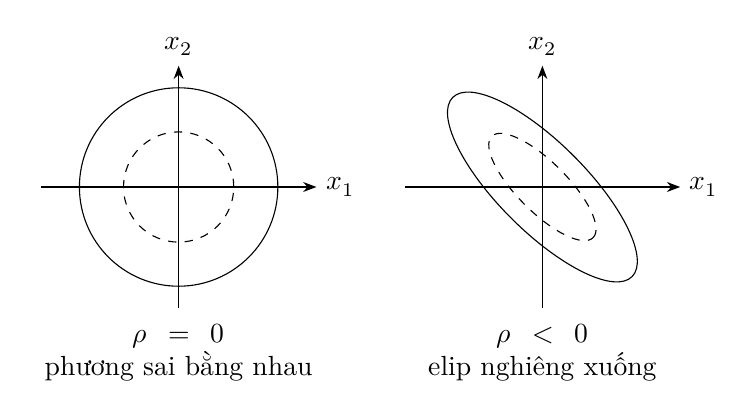
\begin{tikzpicture}[>=Stealth,scale=.7]
 \begin{scope}[xshift=-3.2cm]
 \draw[->] (-2.5,0)--(2.5,0) node[right]{$x_1$};
 \draw[->] (0,-2.2)--(0,2.2) node[above]{$x_2$};
 \draw (0,0) circle (1.8);
 \draw[dashed] (0,0) circle (1);
 \node[align=center,text width=3.6cm] at (0,-3) {$\rho=0$\\phương sai bằng nhau};
 \end{scope}
 \begin{scope}[xshift=3.4cm]
 \draw[->] (-2.5,0)--(2.5,0) node[right]{$x_1$};
 \draw[->] (0,-2.2)--(0,2.2) node[above]{$x_2$};
 \draw[rotate=-45] (0,0) ellipse (2.3 and .8);
 \draw[dashed,rotate=-45] (0,0) ellipse (1.3 and .452);
 \node[align=center,text width=3.6cm] at (0,-3) {$\rho<0$\\elip nghiêng xuống};
 \end{scope}
\end{tikzpicture}
\caption{Tương quan quyết định hướng nghiêng; phương sai và tương quan cùng
quyết định độ dài các trục. Nếu tương quan bằng 0 nhưng phương sai khác nhau,
đường đồng mức vẫn là elip, không nhất thiết là đường tròn.}
\end{figure}

\subsection{Từ khoảng cách đến xác suất: phân phối chi-bình phương}
\begin{result}
Nếu $\mathbf X\sim\N_p(\vmu,\Sigma)$ và $\Sigma$ xác định dương, thì
\begin{equation}
 (\mathbf X-\vmu)'\Sigma^{-1}(\mathbf X-\vmu)\sim\chi^2_p.
 \label{eq:chisqdistance}
\end{equation}
Vì vậy miền
\[
 B=\{\mathbf x:D^2(\mathbf x,\vmu)\le\chi^2_{p;1-\alpha}\}
\]
chứa một quan sát ngẫu nhiên với xác suất $1-\alpha$.
\end{result}
\nguon{Chương 4, §4.2, Result 4.7(a,b), tr.~163--164}

\hieu{Sau khi chuẩn hóa đúng cả độ phân tán lẫn tương quan, ta có $p$
biến chuẩn độc lập với trung bình 0 và phương sai 1. Tổng bình phương của chúng
chính là biến chi-bình phương với $p$ bậc tự do.}
Đây là ý tưởng của phép \emph{làm trắng}; chứng minh được đặt ở
Phụ lục~\ref{app:whitening}.

\begin{example}[Một vùng xác suất 95\%]
Trong hai chiều, $\chi^2_{2;0.95}\approx5.9915$.
Điểm $\mathbf u$ ở ví dụ trên có $D^2=1.1429<5.9915$, còn
$\mathbf v$ có $D^2=8>5.9915$. Điểm thứ nhất nằm trong elip xác suất 95\%,
điểm thứ hai nằm ngoài.
Một điểm nằm ngoài không phải điều bất khả: theo mô hình, khoảng 5\% các
quan sát nằm ngoài vùng này.
\end{example}

\luuy{Đây là vùng cho \emph{một quan sát} khi biết $\vmu,\Sigma$.
Miền tin cậy cho \emph{trung bình tổng thể} khi ước lượng từ mẫu là một bài
toán khác, có $n$, $S$ và ngưỡng Hotelling. Không đổi tên vùng xác suất này
thành miền tin cậy cho $\vmu$.}

\kiemtra{Trong hai chiều, chọn ngưỡng 1 thay vì $\chi^2_{2;0.95}$ có cho
vùng 95\% không? Không: số 1 chỉ ấn định khoảng cách, chưa gắn đúng xác suất.}

\clearpage
\section{Biến đổi tuyến tính, phân phối biên và tính độc lập}
\label{sec:linear}

\subsection{Một công thức kỳ vọng, một công thức hiệp phương sai}
Cho vectơ ngẫu nhiên $\mathbf X$ có trung bình $\vmu$ và hiệp phương sai
$\Sigma$, đặt $\mathbf Y=A\mathbf X+\mathbf d$, trong đó $A$ và
$\mathbf d$ là các hằng số. Khi đó
\begin{equation}
 \E(\mathbf Y)=A\vmu+\mathbf d,\qquad
 \Cov(\mathbf Y)=A\Sigma A'.
 \label{eq:linearmeanvar}
\end{equation}
Hai công thức về moment này đúng ngay cả khi $\mathbf X$ không chuẩn, miễn
các moment tồn tại. Để kết luận \emph{phân phối của $\mathbf Y$ cũng chuẩn},
ta cần giả thiết chuẩn nhiều chiều của $\mathbf X$.

Tại sao $\mathbf d$ không xuất hiện trong hiệp phương sai? Vì
\[
 \mathbf Y-\E(\mathbf Y)=A(\mathbf X-\vmu).
\]
Tịnh tiến mọi giá trị cùng một lượng chỉ đổi tâm, không đổi độ phân tán.
Khi lấy tích ngoài và kỳ vọng, ta được
\[
 \E\bigl[A(\mathbf X-\vmu)(\mathbf X-\vmu)'A'\bigr]=A\Sigma A'.
\]

\subsection{Tổ hợp tuyến tính một biến}
\begin{result}
Nếu $\mathbf X\sim\N_p(\vmu,\Sigma)$, thì với $\mathbf a\in\R^p$,
\begin{equation}
 \mathbf a'\mathbf X\sim\N(\mathbf a'\vmu,\mathbf a'\Sigma\mathbf a).
 \label{eq:unilinear}
\end{equation}
Trường hợp $\mathbf a=0$ cho biến hằng, tức chuẩn suy biến với phương sai 0.
\end{result}
\nguon{Chương 4, §4.2, Result 4.2, tr.~156}

Viết công thức phương sai ra từng thành phần sẽ thấy điều dễ bị bỏ sót:
\[
 \Var\!\left(\sum_i a_iX_i\right)
 =\sum_i a_i^2\sigma_{ii}+2\sum_{i<k}a_i a_k\sigma_{ik}.
\]
Không được chỉ cộng các phương sai nếu các biến chưa được chứng minh không
tương quan. Các hệ số phải được bình phương ở các hạng đường chéo.

\begin{example}[Tổ hợp từ dữ kiện BTVN 1]
Dùng bộ tham số
\begin{equation}
 \vmu=\begin{pmatrix}1\\-1\\2\end{pmatrix},\qquad
 \Sigma=\begin{pmatrix}4&0&-1\\0&5&0\\-1&0&2\end{pmatrix}.
 \label{eq:running3d}
\end{equation}
Bộ này xuất hiện trong Bài 2.1--2.3 của BTVN 1. Ta tự xây dựng tổ hợp
$Y=3X_1-2X_2+X_3$ để minh họa; không dùng lẫn nó với bộ tham số khác của Bài 2.4.

\buoc{1}{Ghi vectơ hệ số}
$\mathbf a=(3,-2,1)'$.
\buoc{2}{Tính trung bình}
$\E(Y)=3(1)-2(-1)+2=7$.
\buoc{3}{Tính phương sai}
\[
 \Sigma\mathbf a=\begin{pmatrix}11\\-10\\-1\end{pmatrix},\qquad
 \mathbf a'\Sigma\mathbf a=3(11)+(-2)(-10)+1(-1)=52.
\]
Cách khai triển cho cùng kết quả:
$9\cdot4+4\cdot5+2+2\cdot3\cdot1\cdot(-1)=52$.
\buoc{4}{Kết luận cả dạng phân phối và tham số}
$Y\sim\N(7,52)$; độ lệch chuẩn là $\sqrt{52}$, không phải 52.
\end{example}

\subsection{Nhiều tổ hợp cùng lúc}
\begin{result}
Nếu $\mathbf X\sim\N_p(\vmu,\Sigma)$ và $A$ có kích thước $q\times p$,
thì
\begin{equation}
 A\mathbf X+\mathbf d\sim\N_q(A\vmu+\mathbf d,A\Sigma A').
 \label{eq:multilinear}
\end{equation}
Nếu $\Sigma$ xác định dương và $A$ có hạng hàng đầy đủ $q$, hiệp phương
sai mới xác định dương. Nếu $A$ thiếu hạng, kết quả là chuẩn suy biến,
không có mật độ thông thường trên toàn bộ $\R^q$.
\end{result}
\nguon{Chương 4, §4.2, Result 4.3, tr.~157; điều kiện hạng được giải thích thêm ở đây}

\begin{example}[Tổng và hiệu]
Với $\mathbf X\sim\N_2((10,20)',\begin{pmatrix}4&3\\3&9\end{pmatrix})$,
đặt $Y_1=X_1-X_2$, $Y_2=X_1+X_2$. Khi đó
\[
 A=\begin{pmatrix}1&-1\\1&1\end{pmatrix},\qquad
 A\vmu=\begin{pmatrix}-10\\30\end{pmatrix}.
\]
Ta tính
\[
 \Var(Y_1)=4+9-2(3)=7,\quad
 \Var(Y_2)=4+9+2(3)=19,
\]
\[
 \Cov(Y_1,Y_2)=\Var(X_1)-\Var(X_2)=4-9=-5.
\]
Vậy $(Y_1,Y_2)'\sim\N_2((-10,30)',\begin{pmatrix}7&-5\\-5&19\end{pmatrix})$.
Tổng và hiệu chưa độc lập; tương quan giữa các biến gốc không phải yếu tố
duy nhất quyết định hiệp phương sai giữa tổng và hiệu.
\end{example}

\subsection{Phân phối biên: chọn biến, không điều kiện hóa}
Phân phối biên mô tả các biến được giữ lại \emph{khi không biết giá trị}
của các biến bị bỏ. Đối với chuẩn nhiều chiều, chỉ cần chọn đúng phần tử
của $\vmu$ và $\Sigma$.

\begin{result}
Nếu phân hoạch
\[
 \mathbf X=\begin{pmatrix}\mathbf X_1\\\mathbf X_2\end{pmatrix},\quad
 \vmu=\begin{pmatrix}\vmu_1\\\vmu_2\end{pmatrix},\quad
 \Sigma=\begin{pmatrix}\Sigma_{11}&\Sigma_{12}\\\Sigma_{21}&\Sigma_{22}\end{pmatrix},
\]
thì $\mathbf X_1\sim\N_{q_1}(\vmu_1,\Sigma_{11})$ và tương tự cho
$\mathbf X_2$.
\end{result}
\nguon{Chương 4, §4.2, Result 4.4, tr.~158--159}

\begin{example}[Chọn các thành phần không liền nhau]
Trong \eqref{eq:running3d}, phân phối của $(X_1,X_3)'$ là
\[
 \N_2\!\left(\begin{pmatrix}1\\2\end{pmatrix},
 \begin{pmatrix}4&-1\\-1&2\end{pmatrix}\right).
\]
Ta chọn hàng và cột 1, 3 theo \emph{cùng thứ tự}. Nếu chọn $(X_3,X_1)'$,
trung bình phải là $(2,1)'$ và hiệp phương sai là
$\begin{pmatrix}2&-1\\-1&4\end{pmatrix}$.
\end{example}

Không cần tích phân mật độ để giải dạng bài này. Một ma trận chọn
$A=\begin{pmatrix}1&0&0\\0&0&1\end{pmatrix}$ trong
\eqref{eq:multilinear} cho ngay kết quả.

\subsection{Độc lập: vai trò quyết định của chuẩn đồng thời}
\begin{result}
Với hai khối thuộc một vectơ \emph{chuẩn đồng thời},
\begin{equation}
 \mathbf X_1\perp\mathbf X_2
 \quad\Longleftrightarrow\quad \Sigma_{12}=0.
 \label{eq:normalindependence}
\end{equation}
Với hai tổ hợp $U=\mathbf a'\mathbf X$, $V=\mathbf b'\mathbf X$,
\begin{equation}
 U\perp V\quad\Longleftrightarrow\quad
 \mathbf a'\Sigma\mathbf b=0.
 \label{eq:linearindependence}
\end{equation}
\end{result}
\nguon{Chương 4, §4.2, Result 4.5, tr.~159--160; phát biểu cho tổ hợp là hệ quả của Results 4.3 và 4.5}

\hieu{Trong mô hình chuẩn, khi khối hiệp phương sai chéo bằng không,
mật độ chung tách được thành tích hai mật độ biên. Đó chính là tính độc lập.
Ngoài mô hình chuẩn, thông tin hiệp phương sai không đủ để mô tả mọi kiểu phụ thuộc.}

Trong \eqref{eq:running3d}, $\Cov(X_1,X_2)=0$ nên $X_1\perp X_2$;
$\Cov(X_1,X_3)=-1$ nên $X_1$ và $X_3$ không độc lập. Hơn nữa,
\[
 \Cov\bigl(X_2,(X_1,X_3)'\bigr)=(0,0)
\]
nên $X_2$ độc lập với \emph{cả vectơ} $(X_1,X_3)'$.
Trong chuẩn nhiều chiều, kết luận này được bảo đảm bởi khối hiệp phương sai.
Trong phân phối tổng quát, độc lập từng cặp không nhất thiết đủ để suy ra
độc lập với cả vectơ.

\begin{example}[Không tương quan nhưng vẫn phụ thuộc]
Cho $Z\sim\N(0,1)$ và $W=Z^2$. Ta có
$\Cov(Z,W)=\E(Z^3)-\E(Z)\E(Z^2)=0$.
Nhưng $W$ do $Z$ quyết định nên không độc lập với $Z$.
Cặp $(Z,W)$ không chuẩn nhiều chiều.
Ví dụ này cho thấy không thể áp dụng \eqref{eq:normalindependence}
chỉ vì một biến có phân phối chuẩn.
\end{example}

Ngay cả việc mỗi biến riêng lẻ đều chuẩn cũng chưa đủ. Cho $Z\sim\N(0,1)$,
cho $B$ độc lập với $Z$, nhận $\pm1$ với xác suất $1/2$; đặt $V=BZ$.
Cả $Z,V$ đều chuẩn và $\Cov(Z,V)=0$, nhưng $|V|=|Z|$ nên chúng phụ thuộc.
Chuẩn \emph{đồng thời} là giả thiết mạnh hơn chuẩn của từng biên.

\subsection{Tìm hệ số để triệt tiêu hiệp phương sai}
\begin{example}[Bài 2.4b của BTVN 1]
Ở bài này, bộ tham số khác với \eqref{eq:running3d}:
\[
 \vmu=(2,-3,1)',\qquad
 \Sigma=\begin{pmatrix}1&1&1\\1&3&2\\1&2&2\end{pmatrix}.
\]
Đặt $\mathbf Z=(X_1,X_3)'$ và $W=X_2-a_1X_1-a_2X_3$.
Đề yêu cầu $X_2\perp W$. Vì cặp này chuẩn đồng thời, ta giải
\[
 \Cov(X_2,W)=3-a_1-2a_2=0.
\]
Toàn bộ nghiệm là $a_1=3-2t$, $a_2=t$, $t\in\R$.
Đây là một phương trình với hai ẩn, nên không có nghiệm duy nhất.
\end{example}

\luuy{Yêu cầu $X_2\perp W$ khác với yêu cầu $\mathbf Z\perp W$.
Trong hồi quy ở phần kế tiếp, ta chọn hệ số để phần dư độc lập với
\emph{các biến dùng dự báo}, chứ không phải với biến cần dự báo.
Hãy đọc đúng hai đại lượng mà đề yêu cầu độc lập.}

\kiemtra{Với chuẩn hai chiều, $\Var(X_1)=\Var(X_2)$, tổng và hiệu có độc
lập không? Có: hiệp phương sai của chúng bằng hiệu hai phương sai, tức 0.}

\clearpage
\section{Phân phối có điều kiện: biết thêm một biến thì điều gì thay đổi?}
\label{sec:conditional}

\subsection{Phân phối biên và có điều kiện trả lời hai câu hỏi khác nhau}
Phân phối biên của chiều cao mô tả một người chọn ngẫu nhiên khi ta chưa
biết cân nặng. Phân phối chiều cao \emph{có điều kiện} tại cân nặng 70 kg
mô tả người trong nhóm có cân nặng đó. Nếu hai đặc điểm liên hệ, biết cân
nặng cung cấp thông tin về chiều cao và làm dự báo bớt bất định.

Ký hiệu $X_1\mid X_2=x_2$ không phải phép chia. Nó nói rằng ta xét phân
phối của $X_1$ sau khi biết giá trị của $X_2$. Vì biến liên tục có xác suất
đúng một điểm bằng 0, công thức có điều kiện được hiểu qua mật độ có điều
kiện, không tính bằng cách chia cho $\Prob(X_2=x_2)$.

\subsection{Công thức hai biến: dễ nhớ qua tương quan}
Với $(X_1,X_2)'$ chuẩn hai chiều, đặt
$\Var(X_1)=\sigma_1^2$, $\Var(X_2)=\sigma_2^2$ và tương quan $\rho$.
Khi $\sigma_2^2>0$,
\begin{align}
 \E(X_1\mid X_2=x_2)
 &=\mu_1+\rho\frac{\sigma_1}{\sigma_2}(x_2-\mu_2),
 \label{eq:cond2mean}\\
 \Var(X_1\mid X_2=x_2)&=\sigma_1^2(1-\rho^2).
 \label{eq:cond2var}
\end{align}
Toàn bộ phân phối có điều kiện là chuẩn với hai tham số này.
\nguon{Chương 4, §4.2, Result 4.6 và Example 4.7, tr.~160--162}

\hieu{Nếu $X_2$ cao hơn trung bình, và $\rho>0$, dự báo $X_1$ cũng dịch
lên. Độ dịch phụ thuộc tương quan và tỉ lệ đơn vị đo.
Thông tin về $X_2$ giải thích được phần $\rho^2$ của phương sai $X_1$;
phần còn lại là $1-\rho^2$.}

Nếu $\rho=0$, trung bình và phương sai không đổi: biết $X_2$ không giúp
dự báo $X_1$ trong mô hình chuẩn. Nếu $|\rho|$ gần 1, phương sai còn lại
nhỏ. Trường hợp $|\rho|=1$ là suy biến, không thuộc mô hình mật độ hai chiều
không suy biến đang xét.

\begin{example}[Một lần cập nhật dự báo]
Giả sử $\vmu=(10,20)'$, $\Sigma=\begin{pmatrix}4&3\\3&9\end{pmatrix}$.
Ta có $\rho=0.5$, $\sigma_1=2$, $\sigma_2=3$.
Khi quan sát $X_2=23$,
\[
 \E(X_1\mid X_2=23)=10+\frac39(23-20)=11,
\]
\[
 \Var(X_1\mid X_2=23)=4-\frac{3^2}{9}=3.
\]
Vậy $X_1\mid X_2=23\sim\N(11,3)$.
Trước khi biết $X_2$, $X_1\sim\N(10,4)$: dự báo đã dịch từ 10 đến 11,
độ lệch chuẩn giảm từ 2 xuống $\sqrt3$.
\end{example}

\begin{figure}[htbp]
\centering
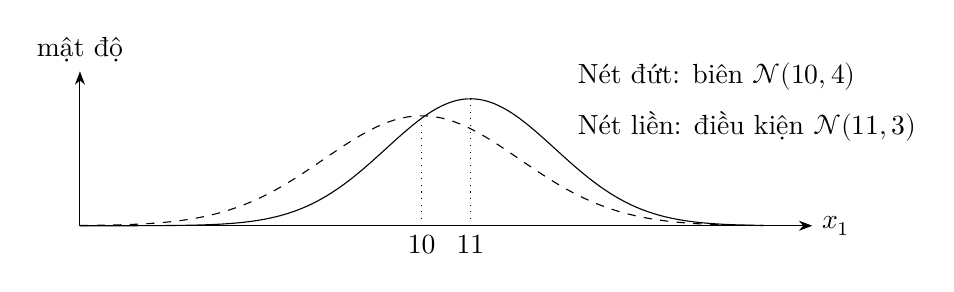
\begin{tikzpicture}[x=.62cm,y=7cm,>=Stealth]
 \draw[->] (3,0)--(18,0) node[right]{$x_1$};
 \draw[->] (3,0)--(3,.28) node[above]{mật độ};
 \draw[domain=3:17,samples=90,smooth,dashed]
 plot (\x,{exp(-((\x-10)^2)/8)/sqrt(8*pi)});
 \draw[domain=3:17,samples=90,smooth]
 plot (\x,{exp(-((\x-11)^2)/6)/sqrt(6*pi)});
 \draw[dotted] (10,0)--(10,.2);
 \draw[dotted] (11,0)--(11,.231);
 \node[below] at (10,0) {10};
 \node[below] at (11,0) {11};
 \node[align=left,anchor=west] at (13,.27) {Nét đứt: biên $\N(10,4)$};
 \node[align=left,anchor=west] at (13,.18) {Nét liền: điều kiện $\N(11,3)$};
\end{tikzpicture}
\caption{Biết $X_2=23$ làm tâm dịch sang phải và phân phối $X_1$ hẹp lại
trong ví dụ. Diện tích dưới mỗi đường vẫn bằng 1.}
\end{figure}

\subsection{Công thức ma trận: dự báo một khối bằng một khối khác}
Phân hoạch vectơ và tham số thành
\[
 \mathbf X=\begin{pmatrix}\mathbf X_1\\\mathbf X_2\end{pmatrix},\quad
 \vmu=\begin{pmatrix}\vmu_1\\\vmu_2\end{pmatrix},\quad
 \Sigma=\begin{pmatrix}\Sigma_{11}&\Sigma_{12}\\\Sigma_{21}&\Sigma_{22}\end{pmatrix}.
\]
Khối $\mathbf X_1$ có $q_1$ thành phần; khối $\mathbf X_2$ có $q_2$ thành
phần. Chỉ số ``1'' ở đây là nhãn \emph{khối}, không nhất thiết chỉ biến
thứ nhất của dữ liệu.

\begin{result}
Nếu vectơ ghép chuẩn và $\Sigma_{22}$ khả nghịch, thì
\begin{equation}
 \mathbf X_1\mid\mathbf X_2=\mathbf x_2
 \sim\N_{q_1}\left(\vmu_{1\mid2},\Sigma_{11\mid2}\right),
 \label{eq:conditional}
\end{equation}
với
\begin{align}
 \vmu_{1\mid2}&=\vmu_1+\Sigma_{12}\Sigma_{22}^{-1}(\mathbf x_2-\vmu_2),
 \label{eq:conditionalmean}\\
 \Sigma_{11\mid2}&=\Sigma_{11}-\Sigma_{12}\Sigma_{22}^{-1}\Sigma_{21}.
 \label{eq:conditionalcov}
\end{align}
\end{result}
\nguon{Chương 4, §4.2, Result 4.6, tr.~160--161; dạng hồi quy (4-9), tr.~163}

Ma trận $B=\Sigma_{12}\Sigma_{22}^{-1}$ có kích thước $q_1\times q_2$
và đóng vai trò hệ số hồi quy. Nó biến độ lệch của khối đã biết thành phần
hiệu chỉnh cho khối cần dự báo.
Khối trừ đi trong \eqref{eq:conditionalcov} là phần phương sai được giải
thích bởi thông tin đó; $\Sigma_{11\mid2}$ còn được gọi là bổ Schur.

Đặc biệt, hiệp phương sai có điều kiện không phụ thuộc \emph{giá trị}
$\mathbf x_2$. Thay $\mathbf x_2$ làm tâm dịch chuyển nhưng không làm
độ phân tán có điều kiện thay đổi. Tính chất này là của mô hình chuẩn;
không suy ra như vậy cho mọi phân phối.

\subsection{Quy trình tính: ghi đúng khối trước khi nhân}
\begin{example}[Dự báo một biến từ hai biến]
Với \eqref{eq:running3d}, tìm $X_1\mid(X_2=x_2,X_3=x_3)$.
\buoc{1}{Đặt khối mục tiêu và khối đã biết}
Đặt $U=X_1$, $\mathbf V=(X_2,X_3)'$.
\buoc{2}{Trích tham số đúng thứ tự}
\[
 \mu_U=1,\quad\vmu_V=\begin{pmatrix}-1\\2\end{pmatrix},\quad
 \Sigma_{UU}=4,\quad\Sigma_{UV}=(0,-1),\quad
 \Sigma_{VV}=\begin{pmatrix}5&0\\0&2\end{pmatrix}.
\]
\buoc{3}{Tính hệ số cập nhật}
\[
 B=(0,-1)\begin{pmatrix}1/5&0\\0&1/2\end{pmatrix}=(0,-1/2).
\]
\buoc{4}{Tính hai tham số}
\[
 \E(U\mid\mathbf V)=1+(0,-1/2)
 \begin{pmatrix}x_2+1\\x_3-2\end{pmatrix}=2-\frac{x_3}{2},
\]
\[
 \Var(U\mid\mathbf V)=4-(0,-1/2)(0,-1)'=\frac72.
\]
Vậy $X_1\mid(X_2=x_2,X_3=x_3)\sim\N(2-x_3/2,7/2)$.
Giá trị $x_2$ biến mất vì $X_2$ độc lập với cả $(X_1,X_3)'$.
\end{example}

Nếu chỉ biết $X_3=x_3$, ta vẫn nhận được đúng phân phối trên. Khi
$x_3=4$, trung bình có điều kiện bằng 0. Không có mâu thuẫn với trung bình
biên bằng 1: đó là trung bình trên tất cả các giá trị của $X_3$, còn ở đây
ta đã giới hạn vào một nhóm có $X_3=4$.

\subsection{Phần dư hồi quy và tính độc lập}
Đặt phần dư đã trừ trung bình
\[
 \mathbf R=\mathbf X_1-\vmu_1-B(\mathbf X_2-\vmu_2),
 \qquad B=\Sigma_{12}\Sigma_{22}^{-1}.
\]
Ta có $\E(\mathbf R)=0$ và
\[
 \Cov(\mathbf R,\mathbf X_2)=\Sigma_{12}-B\Sigma_{22}=0.
\]
Vì $(\mathbf R,\mathbf X_2)$ chuẩn đồng thời, $\mathbf R\perp\mathbf X_2$.
Do đó khi biết $\mathbf X_2$, phần dư vẫn có cùng phân phối; điều kiện hóa
chỉ biến $B(\mathbf X_2-\vmu_2)$ thành một độ dịch tâm xác định.
Đây là cách suy ra công thức có điều kiện mà không cần tính tích phân.

\luuy{Ở đây các hệ số $B$ tính từ tham số tổng thể đã biết. Đây là tính
chất của phân phối, chưa phải bài toán ước lượng hệ số hồi quy từ mẫu.
Không tự thay bậc tự do của hồi quy vào công thức này.}

\kiemtra{Có thể lấy ma trận hiệp phương sai biên $\Sigma_{11}$ làm
hiệp phương sai có điều kiện không? Chỉ khi phần hiệu chỉnh bằng 0,
chẳng hạn hai khối độc lập.}

\clearpage
\section{Phân phối mẫu: từ một quan sát đến thống kê của cả mẫu}
\label{sec:sampling}

\subsection{Trung bình mẫu và hiệp phương sai mẫu}
Cho $\mathbf X_1,\ldots,\mathbf X_n$ là mẫu iid, mỗi quan sát có $p$ biến.
Định nghĩa
\begin{align}
 \Xbar&=\frac1n\sum_{j=1}^n\mathbf X_j,
 \label{eq:samplemean}\\
 S&=\frac1{n-1}\sum_{j=1}^n
 (\mathbf X_j-\Xbar)(\mathbf X_j-\Xbar)'.
 \label{eq:samplecov}
\end{align}
Mỗi phần tử $s_{ik}$ là hiệp phương sai mẫu của hai cột $i,k$.
Ký hiệu $S$ dùng cho cả thống kê ngẫu nhiên và ma trận giá trị đã tính;
ngữ cảnh sẽ phân biệt. $\Xbar$ ngẫu nhiên trước khi lấy mẫu, còn $\xbar$
là giá trị cụ thể sau khi lấy mẫu.

\begin{example}[Tính từ bảng bốn quan sát]
Với $\mathbf D=\begin{pmatrix}2&12\\8&9\\6&9\\8&10\end{pmatrix}$,
\[
 \xbar=\begin{pmatrix}6\\10\end{pmatrix},\qquad
 \mathbf D_{\mathrm{centered}}=
 \begin{pmatrix}-4&2\\2&-1\\0&-1\\2&0\end{pmatrix}.
\]
Đường chéo và hiệp phương sai lần lượt là
\[
 s_{11}=\frac{16+4+0+4}{3}=8,\quad
 s_{22}=\frac{4+1+1+0}{3}=2,
\]
\[
 s_{12}=\frac{(-4)(2)+(2)(-1)+(0)(-1)+(2)(0)}3=-\frac{10}3.
\]
Do đó
\begin{equation}
 S=\begin{pmatrix}8&-10/3\\-10/3&2\end{pmatrix},\qquad
 S^{-1}=\frac1{22}\begin{pmatrix}9&15\\15&36\end{pmatrix}.
 \label{eq:sample4}
\end{equation}
Ma trận tích $\mathbf D_{\mathrm{centered}}'
\mathbf D_{\mathrm{centered}}$ cho đúng $(n-1)S$.
\end{example}

\subsection{Phân phối của trung bình mẫu chuẩn}
\begin{result}
Nếu $\mathbf X_j\overset{\mathrm{iid}}\sim\N_p(\vmu,\Sigma)$, thì
\begin{equation}
 \Xbar\sim\N_p\left(\vmu,\frac{\Sigma}{n}\right).
 \label{eq:samplemeandist}
\end{equation}
\end{result}
\nguon{Chương 4, §4.4, công thức (4-23), tr.~174}

Kỳ vọng vẫn bằng $\vmu$, còn hiệp phương sai giảm $n$ lần.
Điều này do các quan sát độc lập: các hiệp phương sai giữa đối tượng khác
nhau bằng 0. Với một tổ hợp $\mathbf a'\Xbar$, phương sai là
$\mathbf a'\Sigma\mathbf a/n$.

\hieu{Nếu lấy lại nhiều mẫu, trung bình của các mẫu sẽ tụ quanh cùng một
vectơ trung bình tổng thể. Mẫu càng lớn, đám mây các trung bình mẫu càng nhỏ.
Các quan sát riêng lẻ vẫn có độ phân tán $\Sigma$; chúng không tự trở nên
ít biến thiên chỉ vì ta lấy thêm dữ liệu.}

Với $p=2$, $n=25$ và $\Sigma=\diag(4,9)$, độ lệch chuẩn của hai thành
phần trung bình mẫu là $2/5$ và $3/5$, còn độ lệch chuẩn của quan sát là 2
và 3. Cần giữ rõ ta đang xét loại đại lượng nào.

\subsection{Dạng toàn phương khi biết hiệp phương sai tổng thể}
Từ \eqref{eq:samplemeandist}, $\sqrt n(\Xbar-\vmu)\sim\N_p(0,\Sigma)$.
Áp dụng kết quả khoảng cách Mahalanobis cho vectơ này:
\begin{equation}
 n(\Xbar-\vmu)'\Sigma^{-1}(\Xbar-\vmu)\sim\chi^2_p.
 \label{eq:knowncovmean}
\end{equation}
Đây là kết quả \emph{chính xác} trong mẫu chuẩn khi dùng $\Sigma$ thật,
ngay cả ở mẫu nhỏ. Trong Bài 2.9 với $n=60,p=4$, trung bình mẫu có
hiệp phương sai $\Sigma/60$; dạng toàn phương của một quan sát và dạng
\eqref{eq:knowncovmean} đều có phân phối $\chi^2_4$.
Không có mâu thuẫn: hệ số $n$ bù cho việc trung bình mẫu biến thiên ít hơn.
\nguon{Hệ quả của Chương 4, Result 4.7, tr.~163, và (4-23), tr.~174}

Nếu thay $\Sigma^{-1}$ bằng $S^{-1}$, ma trận chuẩn hóa cũng ngẫu nhiên.
Khi đó không thể giữ nguyên kết luận chi-bình phương chính xác; cần
phân phối Hotelling hữu hạn hoặc xấp xỉ mẫu lớn. Đây là điểm phân biệt
quan trọng giữa các câu của Bài 2.9.

\subsection{Wishart: mở rộng chi-bình phương từ số sang ma trận}
Trong một chiều, tổng bình phương các biến chuẩn độc lập cho phân phối
chi-bình phương. Trong nhiều chiều, thay bình phương $Z^2$ bằng tích ngoài
$\mathbf Z\mathbf Z'$, ta có phân phối Wishart.

\begin{definition}
Nếu $\mathbf Z_1,\ldots,\mathbf Z_\nu$ iid $\N_p(0,\Sigma)$, thì
\[
 W=\sum_{j=1}^\nu\mathbf Z_j\mathbf Z_j'
 \sim W_{p,\nu}(\Sigma).
\]
$p$ là kích thước ma trận, $\nu$ là số bậc tự do, $\Sigma$ là ma trận
tham số tỉ lệ. Một số tài liệu viết $W_p(\Sigma,\nu)$ cho cùng phân phối.
\end{definition}
\nguon{Chương 4, §4.4, định nghĩa (4-22), tr.~174}

\begin{result}
Với mẫu iid chuẩn nhiều chiều,
\begin{equation}
 (n-1)S\sim W_{p,n-1}(\Sigma),\qquad \Xbar\perp S.
 \label{eq:wishart}
\end{equation}
\end{result}
\nguon{Chương 4, §4.4, công thức (4-23), tr.~174}

\hieu{Trung bình mẫu cung cấp thông tin về vị trí; hiệp phương sai mẫu
cung cấp thông tin về độ phân tán. Trong mô hình chuẩn, hai phần thông tin
này ngẫu nhiên độc lập với nhau. Tính chất đặc biệt đó cho phép xây dựng
phân phối kiểm định chính xác ở phần tiếp theo.}

Vì sao bậc tự do là $n-1$? Các độ lệch cộng lại bằng 0:
$\sum_j(\mathbf X_j-\Xbar)=0$. Sau khi biết $n-1$ độ lệch, độ lệch còn
lại đã được xác định. Các độ lệch này không iid, nhưng có thể đổi hệ tọa độ
giữa các quan sát để viết tổng tích ngoài thành tổng của $n-1$ vectơ chuẩn
độc lập. Phụ lục~\ref{app:wishart} mô tả phép đổi đó.

Với $p=1$, Wishart thu về
\[
 \frac{(n-1)s^2}{\sigma^2}\sim\chi^2_{n-1},
\]
nên đây thực sự là mở rộng của kết quả một chiều.

\subsection{Khi nào \texorpdfstring{$S$}{S} có nghịch đảo?}
Hạng của ma trận dữ liệu đã trừ trung bình không vượt quá $n-1$. Do đó
\[
 \operatorname{rank}(S)\le\min(p,n-1).
\]
Nếu $n\le p$, $S$ chắc chắn suy biến. Nếu mẫu iid chuẩn, $\Sigma$ xác định
dương và $n>p$, thì $S$ khả nghịch với xác suất 1. Trong dữ liệu thực,
biến lặp lại hoặc quan hệ tuyến tính chính xác vẫn có thể gây suy biến.

\luuy{Điều kiện $n>p$ là cần thiết để dùng nghịch đảo hiệp phương sai
mẫu trong kiểm định cổ điển. Nó không tự bảo đảm dữ liệu bất kỳ không có
cột trùng hay cột hằng. Cũng không nên thay $S^{-1}$ bằng nghịch đảo giả rồi
giữ nguyên ngưỡng $F$; đó là một phương pháp khác.}

\subsection{Thiết lập MLE: đi từ mật độ đến ước lượng}
\label{sec:mle_derivation}
Ước lượng hợp lý cực đại (maximum likelihood estimation, MLE) chọn các
tham số làm dữ liệu \emph{đã quan sát} có mật độ chung lớn nhất. Khi tìm
MLE, các $\mathbf x_j$ là số đã biết; $\vmu,\Sigma$ là các biến cần tối ưu.
Ta không tìm tham số có xác suất lớn nhất, vì tham số ở đây không được
đặt một phân phối xác suất.

Giả sử mẫu iid $\N_p(\vmu,\Sigma)$ và $\Sigma\succ0$. Để có nghiệm MLE
không suy biến, giả sử ma trận tổng tích ngoài quanh $\xbar$ xác định dương.
Trong mẫu chuẩn với hiệp phương sai tổng thể xác định dương, $n>p$ bảo
đảm điều này với xác suất 1; đối với bảng số cụ thể vẫn phải kiểm tra hạng.

\buoc{1}{Viết hàm hợp lý và log-hợp lý}
Tính độc lập cho phép nhân $n$ mật độ:
\begin{equation}
 L(\vmu,\Sigma)=(2\pi)^{-np/2}|\Sigma|^{-n/2}
 \exp\!\left[-\frac12\sum_{j=1}^n
 (\mathbf x_j-\vmu)'\Sigma^{-1}(\mathbf x_j-\vmu)\right].
 \label{eq:mlelikelihood}
\end{equation}
Logarit là hàm tăng, nên cực đại $L$ cũng là cực đại $\ell=\log L$:
\begin{equation}
 \ell(\vmu,\Sigma)=-\frac{np}2\log(2\pi)-\frac n2\log|\Sigma|
 -\frac12\sum_{j=1}^n(\mathbf x_j-\vmu)'\Sigma^{-1}(\mathbf x_j-\vmu).
 \label{eq:mleloglikelihood}
\end{equation}
Logarit chuyển tích thành tổng, làm phép tối ưu dễ xử lý hơn.
\nguon{Chương 4, §4.3, mật độ mẫu (4-11), tr.~168; hàm hợp lý (4-16), tr.~170}

\buoc{2}{Tách phần phụ thuộc trung bình và tìm $\widehat{\vmu}$}
Đặt
\[
 A=\sum_j(\mathbf x_j-\xbar)(\mathbf x_j-\xbar)'=(n-1)S.
\]
Vì $\sum_j(\mathbf x_j-\xbar)=0$, hai hạng chéo triệt tiêu khi khai triển:
\begin{equation}
 \sum_j(\mathbf x_j-\vmu)(\mathbf x_j-\vmu)'
 =A+n(\xbar-\vmu)(\xbar-\vmu)'.
 \label{eq:mlescatterdecomposition}
\end{equation}
Trace, ký hiệu $\tr(B)$, là tổng các phần tử đường chéo của ma trận vuông.
Với vectơ $\mathbf u$, ta có
$\mathbf u'B\mathbf u=\tr(B\mathbf u\mathbf u')$; do đó
\begin{align}
 \ell(\vmu,\Sigma)
 &=K-\frac n2\log|\Sigma|-\frac12\tr(\Sigma^{-1}A)
 \notag\\[-2pt]
 &\qquad-\frac n2(\xbar-\vmu)'\Sigma^{-1}(\xbar-\vmu),
 \label{eq:mlemeansplit}
\end{align}
trong đó $K=-np\log(2\pi)/2$ không phụ thuộc tham số.

Với $\Sigma$ cố định, chỉ hạng cuối phụ thuộc $\vmu$. Vì
$\Sigma^{-1}\succ0$, hạng toàn phương không âm, bằng 0 duy nhất khi
$\vmu=\xbar$. Nó mang dấu trừ trong log-hợp lý, nên
\begin{equation}
 \widehat{\vmu}=\xbar.
 \label{eq:mlemeanhat}
\end{equation}
Kết quả đúng với \emph{mọi} $\Sigma\succ0$ cố định, nên có thể thay
$\vmu=\xbar$ trước rồi tối ưu theo $\Sigma$.
\nguon{Chương 4, §4.3, phân rã (4-14), tr.~169; Result 4.11, tr.~171--172}

\buoc{3}{Đổi biến để tìm ma trận hiệp phương sai}
Đặt $\Theta=\Sigma^{-1}$, gọi là \emph{ma trận độ chính xác}. Đây là
phép đổi biến một-một trên các ma trận xác định dương. Vì
$\log|\Sigma|=-\log|\Theta|$, log-hợp lý sau khi chọn trung bình là
\begin{equation}
 \ell(\xbar,\Theta)=K+\frac n2\log|\Theta|-\frac12\tr(\Theta A).
 \label{eq:mleprecision}
\end{equation}
Ý nghĩa của hai hạng: $\log|\Theta|$ thưởng cho độ phân tán nhỏ, còn
$\tr(\Theta A)$ phạt nếu độ phân tán quá nhỏ so với các độ lệch thực tế.
Cực đại cân bằng hai hạng đó.

Để đạo hàm, dùng hai quy tắc ma trận
\[
 d\log|\Theta|=\tr(\Theta^{-1}d\Theta),\qquad
 d\tr(\Theta A)=\tr(A\,d\Theta).
\]
Ký hiệu $d\Theta$ là một thay đổi nhỏ của ma trận, không phải vectơ
tịnh tiến $\mathbf d$ dùng ở phần biến đổi dữ liệu. Hai quy tắc trên là
bản mở rộng của $(\log\theta)'=1/\theta$ và $(a\theta)'=a$.
Từ \eqref{eq:mleprecision},
\[
 d\ell=\frac12\tr\bigl[(n\Theta^{-1}-A)d\Theta\bigr].
\]
Tại điểm dừng, biểu thức phải bằng 0 theo mọi hướng thay đổi đối xứng,
nên $n\Theta^{-1}-A=0$. Suy ra
\begin{equation}
 \widehat\Sigma=\widehat\Theta^{-1}=\frac An
 =\frac1n\sum_j(\mathbf x_j-\xbar)(\mathbf x_j-\xbar)'
 =\frac{n-1}{n}S.
 \label{eq:mlecov}
\end{equation}
Đó là nguồn gốc của mẫu số $n$; ta không chọn mẫu số theo ý thích.

\buoc{4}{Kiểm tra điểm dừng thực sự là cực đại}
Đạo hàm bằng 0 chưa đủ để kết luận. Với hướng đối xứng $H\ne0$, đạo
hàm bậc hai theo đường $\Theta+tH$ là
\[
 \frac{d^2}{dt^2}\ell(\xbar,\Theta+tH)\bigg|_{t=0}
 =-\frac n2\tr(\Theta^{-1}H\Theta^{-1}H)<0.
\]
Thật vậy, trace trong vế phải bằng tổng bình phương các trị riêng của
ma trận đối xứng $\Theta^{-1/2}H\Theta^{-1/2}$, nên dương khi $H\ne0$.
Log-hợp lý là hàm lõm nghiêm ngặt theo $\Theta$ trên miền xác định dương,
vì vậy điểm dừng tìm được là cực đại duy nhất. Kết hợp Bước 2, đây cũng
là cực đại đồng thời theo cả trung bình và hiệp phương sai.
\nguon{Kết quả MLE: Chương 4, §4.3, Result 4.11, tr.~171--172.
 Sách chứng minh bằng Result 4.10; ở đây dùng dẫn xuất tương đương theo ma trận độ chính xác}

\hieu{Trung bình mẫu đặt tâm tốt nhất của đám mây. Hiệp phương sai MLE
khớp độ phân tán quanh tâm đó bằng trung bình của các tích ngoài.
Tối ưu theo ma trận độ chính xác giúp nhìn rõ nghiệm và kiểm tra cực đại.}

\subsection{MLE khác ước lượng không chệch như thế nào?}
Thay các giá trị quan sát bằng biến ngẫu nhiên, các công thức MLE trở
thành các \emph{ước lượng} $\widehat{\vmu}=\Xbar$ và
$\widehat\Sigma=(n-1)S/n$. Khi đã thay số, đó là các \emph{giá trị ước lượng}.
Ta có
\[
 \E(S)=\Sigma,\qquad
 \E(\widehat\Sigma)=\frac{n-1}{n}\Sigma.
\]
$S$ không chệch; MLE hiệp phương sai bị chệch xuống ở mẫu hữu hạn.
MLE tối ưu hàm hợp lý, không tối ưu tiêu chí ``không chệch''. Hai mục
tiêu khác nhau, nên cho mẫu số khác nhau. Khi $n$ lớn, tỉ lệ $(n-1)/n$
tiến về 1 và khác biệt giảm.

\begin{example}[Tính MLE từ mẫu bốn quan sát]
Với $\xbar=(6,10)'$, $S$ trong \eqref{eq:sample4}, $n=4$,
\[
 A=3S=\begin{pmatrix}24&-10\\-10&6\end{pmatrix},\quad
 \widehat{\vmu}=\begin{pmatrix}6\\10\end{pmatrix},\quad
 \widehat\Sigma=\frac A4=\begin{pmatrix}6&-2.5\\-2.5&1.5\end{pmatrix}.
\]
Ta có $|\widehat\Sigma|=2.75>0$ và $\widehat\Theta=4A^{-1}$,
kiểm tra được $4\widehat\Theta^{-1}=A$.
Để kiểm định Hotelling, ta dùng $S$, không thế $\widehat\Sigma$ vào
công thức $n\mathbf r'S^{-1}\mathbf r$ mà giữ nguyên ngưỡng $F$.
Để thiết lập tỷ số hợp lý, ta dùng đúng MLE $\widehat\Sigma$.
\end{example}

\luuy{Nếu $A$ suy biến, $A/n$ không thuộc miền $\Sigma\succ0$.
Không có MLE hữu hạn trong mô hình chuẩn không suy biến này: có thể
co phương sai về 0 theo một hướng không có độ lệch quan sát, khiến hàm
hợp lý tăng không giới hạn. Tình huống này xảy ra khi $n\le p$, hoặc
do các cột phụ thuộc tuyến tính. Phụ lục~\ref{app:mle_global} giải thích
bằng trị riêng, đồng thời kiểm tra cực đại mà không dùng đạo hàm ma trận.}

\kiemtra{Dùng cùng một mẫu, $S$ và MLE hiệp phương sai có thể khác nhau
không? Có; MLE bằng $(n-1)S/n$. MLE trung bình có cần biết trước
$\Sigma$ không? Không, nghiệm $\xbar$ đúng với mọi $\Sigma\succ0$.}


\subsection{Không chuẩn nhưng mẫu lớn: luật số lớn và CLT}
Giả sử mẫu iid từ tổng thể bất kỳ, có trung bình $\vmu$ và hiệp phương
sai hữu hạn $\Sigma$, với $p$ cố định. Khi $n\to\infty$,
\begin{equation}
 \Xbar\xrightarrow{P}\vmu,\qquad S\xrightarrow{P}\Sigma.
 \label{eq:lln}
\end{equation}
Ký hiệu $\xrightarrow{P}$ là hội tụ theo xác suất: xác suất sai lệch lớn
hơn bất kỳ mức dương cho trước tiến về 0.
\nguon{Chương 4, §4.5, Result 4.12 và công thức (4-26), (4-27), tr.~175}

Định lý giới hạn trung tâm nhiều chiều nói rằng
\begin{equation}
 \sqrt n(\Xbar-\vmu)\xrightarrow{d}\N_p(0,\Sigma).
 \label{eq:clt}
\end{equation}
Ký hiệu $\xrightarrow{d}$ là hội tụ về phân phối. Công thức này mô tả
hình dạng giới hạn của sai lệch đã nhân $\sqrt n$; không nói mỗi quan sát
$\mathbf X_j$ trở thành chuẩn khi tăng $n$.
\nguon{Chương 4, §4.5, Result 4.13, tr.~176}

Nếu $\Sigma$ xác định dương, Slutsky cho phép thay $\Sigma$ bằng ước lượng
nhất quán $S$ trong dạng toàn phương:
\begin{equation}
 n(\Xbar-\vmu)'S^{-1}(\Xbar-\vmu)\xrightarrow{d}\chi^2_p.
 \label{eq:slutsky}
\end{equation}
\nguon{Chương 4, §4.5, công thức (4-28), tr.~176; ứng dụng ở Result 5.4, tr.~235}

\hieu{CLT cho hình dạng chuẩn ở giới hạn, luật số lớn cho phép ước lượng
độ phân tán, và Slutsky nối hai kết quả. Không cần giả thiết chuẩn tổng thể
cho kết quả giới hạn này, nhưng cần iid, moment hữu hạn và hiệp phương sai
không suy biến.}

Trong mẫu chuẩn, các kết quả Wishart và độc lập là \emph{chính xác ở mẫu
hữu hạn}; trong tổng thể bất kỳ, chúng không tự được khôi phục chỉ vì mẫu
lớn. Ta chỉ dùng kết quả xấp xỉ thích hợp. Cách chọn sẽ được tóm tắt ở
Phần~\ref{sec:large}.

\kiemtra{Có cần $n-p\ge30$ để $S\xrightarrow{P}\Sigma$ đúng không?
Không. Hội tụ là phát biểu khi $n\to\infty$; một ngưỡng mẫu hữu hạn không
phải giả thiết của luật số lớn.}

\clearpage
\section{Kiểm định Hotelling \texorpdfstring{$T^2$}{T²}: trung bình có khác giả thuyết?}
\label{sec:hotelling}

\subsection{Vì sao không kiểm định riêng từng biến?}
Giả sử cần kiểm tra $H_0:\vmu=(\mu_{01},\mu_{02})'$. Làm hai kiểm định
$t$ mức 5\% không tạo ra một kiểm định chung mức 5\%: xác suất có ít nhất
một bác bỏ sai có thể lớn hơn 5\%. Hơn nữa, một hướng như $X_1-X_2$ có
thể ít biến thiên dù từng biến riêng có phương sai lớn. Sự khác biệt theo
hướng đó có thể bị bỏ qua nếu chỉ kiểm định từng thành phần.

Hotelling $T^2$ dùng \emph{toàn bộ} ma trận hiệp phương sai để đánh giá
vectơ chênh lệch giữa trung bình mẫu và giả thuyết. Nó là phép mở rộng
trực tiếp của
\[
 t^2=n(\bar x-\mu_0)^2/s^2.
\]
\nguon{Chương 5, §5.2, tr.~210--212, công thức (5-1)--(5-4)}

\subsection{Thống kê và phân phối chính xác}
Ta xét giả thuyết hai phía
\[
 H_0:\vmu=\vmu_0,\qquad H_1:\vmu\ne\vmu_0.
\]
\begin{definition}
Thống kê Hotelling một mẫu là
\begin{equation}
 T^2=n(\Xbar-\vmu_0)'S^{-1}(\Xbar-\vmu_0).
 \label{eq:t2}
\end{equation}
\end{definition}
\nguon{Chương 5, §5.2, công thức (5-4), tr.~211}

\hieu{$T^2$ là bình phương khoảng cách từ trung bình mẫu đến vectơ
giả thuyết, đo bằng hiệp phương sai của \emph{trung bình mẫu}, ước lượng
bởi $S/n$. Giá trị lớn nghĩa là chênh lệch quan sát lớn so với sai số lấy mẫu.}

\begin{result}
Nếu $\mathbf X_1,\ldots,\mathbf X_n$ iid $\N_p(\vmu,\Sigma)$,
$\Sigma$ xác định dương, $n>p$, thì dưới $H_0$,
\begin{equation}
 F_{\mathrm{obs}}=\frac{n-p}{p(n-1)}T^2\sim F_{p,n-p}.
 \label{eq:t2F}
\end{equation}
Bác bỏ $H_0$ mức $\alpha$ nếu
\begin{equation}
 T^2>c_T^2,\qquad
 c_T^2=\frac{p(n-1)}{n-p}F_{p,n-p;1-\alpha}.
 \label{eq:t2critical}
\end{equation}
\end{result}
\nguon{Chương 5, §5.2, công thức (5-5)--(5-7), tr.~212}

Một cách tương đương là so sánh $F_{\mathrm{obs}}$ với phân vị $F$.
Không so trực tiếp $T^2$ với phân vị $F$ mà bỏ hệ số chuyển đổi.
Giá trị p là
\[
 \text{p-value}=1-G_{p,n-p}\!\left(\frac{n-p}{p(n-1)}T^2_{\mathrm{obs}}\right),
\]
trong đó $G_{p,n-p}$ là hàm phân phối tích lũy $F$.
Phần mềm thường có hàm survival function để tính đuôi phải ổn định hơn
phép trừ $1-G$ khi xác suất rất nhỏ.

\subsection{Ví dụ mẫu nhỏ: thực hiện trọn quy trình}
\begin{example}[Bài 3.1 của BTVN 2, tương ứng Exercise 5.1 trong sách]
Với dữ liệu bốn quan sát ở Phần~\ref{sec:sampling}, kiểm định
$\vmu_0=(7,11)'$ tại $\alpha=0.05$, giả sử mẫu iid chuẩn hai chiều.
\buoc{1}{Xác định kích thước và thống kê mẫu}
$n=4$, $p=2$, $\xbar=(6,10)'$, $S$ và $S^{-1}$ như
\eqref{eq:sample4}. Vì $|S|=44/9>0$, nghịch đảo tồn tại.
\buoc{2}{Tính vectơ chênh lệch}
$\mathbf d=\xbar-\vmu_0=(-1,-1)'$.
\buoc{3}{Tính thống kê}
\[
 T^2=\frac4{22}(-1,-1)
 \begin{pmatrix}9&15\\15&36\end{pmatrix}
 \begin{pmatrix}-1\\-1\end{pmatrix}
 =\frac{150}{11}\approx13.6364.
\]
\buoc{4}{Chọn phân phối và ngưỡng đúng}
\[
 F_{\mathrm{obs}}=\frac{4-2}{2(4-1)}T^2=
 \frac{T^2}{3}=\frac{50}{11}\approx4.5455.
\]
Dưới $H_0$, $F_{\mathrm{obs}}\sim F_{2,2}$.
Phân vị $F_{2,2;0.95}=19$, nên $c_T^2=3\cdot19=57$.
\buoc{5}{Ra quyết định và diễn giải}
$13.6364<57$: chưa bác bỏ $H_0$ ở mức 5\%.
Giá trị p bằng $11/61\approx0.1803$.
Chưa đủ bằng chứng để nói vectơ trung bình tổng thể khác $(7,11)'$.
\end{example}

Mẫu rất nhỏ làm $S$ có độ bất định lớn, nên ngưỡng kiểm định cao.
Nếu sai lầm dùng $\chi^2_{2;0.95}=5.9915$, ta sẽ bác bỏ ở ví dụ này,
trái với kiểm định chính xác. Đây không phải chi tiết nhỏ về làm tròn:
lựa chọn phân phối thay đổi kết luận.
\nguon{Dữ kiện Exercise 5.1, Chương 5; lý thuyết §5.2. Phép tính được kiểm tra độc lập}

\subsection{Kiểm tra bằng trường hợp một chiều}
Đặt $p=1$ trong \eqref{eq:t2F}:
\[
 \frac{n-1}{n-1}T^2=T^2\sim F_{1,n-1}.
\]
Mà $t_{n-1}^2\sim F_{1,n-1}$, nên kiểm định Hotelling thu về kiểm định
$t$ hai phía. Ngưỡng $F_{1,n-1;1-\alpha}$ bằng
$t_{n-1;1-\alpha/2}^2$.

\kiemtra{Trong ví dụ mẫu nhỏ, thống kê nào có phân phối $F_{2,2}$:
$T^2$ hay $T^2/3$? Đáp án: $T^2/3$.}

\subsection{Tính bất biến: đổi đơn vị đo không đổi kết luận}
\label{sec:invariance_proof}
Cho $\mathbf Y_j=C\mathbf X_j+\mathbf d$ với $C$ vuông khả nghịch.
Biến đổi đồng thời
\[
 \bar{\mathbf y}=C\xbar+\mathbf d,\quad S_Y=CS_XC',\quad
 \vmu_{Y,0}=C\vmu_0+\mathbf d.
\]
Khi đó
\begin{equation}
 T_Y^2=T_X^2.
 \label{eq:invariance}
\end{equation}
Đổi mét sang centimét, đổi thang nhiệt độ hoặc chọn một hệ trục khả nghịch
chỉ biểu diễn cùng thông tin theo cách khác. Chuẩn hóa chênh lệch bằng
hiệp phương sai làm các hệ số đổi đơn vị triệt tiêu.
\nguon{Chương 5, §5.2, phép biến đổi (5-9) và lập luận bất biến, tr.~215--216}

\buoc{1}{Chứng minh các thống kê mẫu biến đổi đồng bộ}
Tính trung bình hai vế của $\mathbf y_j=C\mathbf x_j+\mathbf d$ cho
$\bar{\mathbf y}=C\xbar+\mathbf d$. Do đó
\[
 \mathbf y_j-\bar{\mathbf y}=C(\mathbf x_j-\xbar).
\]
Thế vào định nghĩa hiệp phương sai mẫu:
\begin{align*}
 S_Y&=\frac1{n-1}\sum_j
 C(\mathbf x_j-\xbar)(\mathbf x_j-\xbar)'C'\\
 &=C\left[\frac1{n-1}\sum_j
 (\mathbf x_j-\xbar)(\mathbf x_j-\xbar)'\right]C'=CS_XC'.
\end{align*}
Giả thuyết cũng đổi hệ tọa độ:
$\vmu_{Y,0}=C\vmu_0+\mathbf d$.
Đặt $\mathbf r=\xbar-\vmu_0$, ta nhận được độ lệch mới
\[
 \bar{\mathbf y}-\vmu_{Y,0}=C\mathbf r.
\]
Phần tịnh tiến triệt tiêu vì xuất hiện ở cả hai trung bình.

\buoc{2}{Thiết lập nghịch đảo của hiệp phương sai mới}
Với tích các ma trận khả nghịch, nghịch đảo lấy theo thứ tự ngược lại:
\[
 (CS_XC')^{-1}=(C')^{-1}S_X^{-1}C^{-1}.
\]
Có thể kiểm tra bằng cách nhân với $CS_XC'$: các cặp
$C'(C')^{-1}$, $S_XS_X^{-1}$, $CC^{-1}$ lần lượt triệt tiêu và cho $I_p$.

\buoc{3}{Thế vào thống kê Hotelling}
\begin{align*}
 T_Y^2
 &=n(C\mathbf r)'(CS_XC')^{-1}(C\mathbf r)\\
 &=n\mathbf r'C'(C')^{-1}S_X^{-1}C^{-1}C\mathbf r\\
 &=n\mathbf r'S_X^{-1}\mathbf r=T_X^2.
\end{align*}
Các hệ số đổi tọa độ xuất hiện trong cả độ lệch lẫn hiệp phương sai,
nên triệt tiêu khi chuẩn hóa. Đây là chứng minh bất biến của \emph{giá
trị thống kê}, không chỉ của dạng công thức.

\buoc{4}{Suy ra bất biến của giá trị p và quyết định kiểm định}
$C$ là ma trận $p\times p$ khả nghịch nên không thay đổi $n$ hoặc $p$.
Hệ số chuyển sang $F$, số bậc tự do và ngưỡng $c_T^2$ đều giữ nguyên.
Vì vậy cùng một $T^2$ cho cùng giá trị p và cùng quyết định bác bỏ hay
chưa bác bỏ. Dưới giả thiết mẫu chuẩn, mẫu biến đổi vẫn chuẩn và có
hiệp phương sai $C\Sigma C'\succ0$, nên phân phối kiểm định chính xác
vẫn áp dụng được.

\hieu{Nếu đổi đơn vị đo hoặc trộn các biến theo một cách có thể hoàn
tác, ta vẫn giữ toàn bộ thông tin về giả thuyết. Kiểm định vectơ trung
bình cần cho cùng kết luận trong hai cách biểu diễn đó.}

Đẳng thức đại số $T_Y^2=T_X^2$ không cần giả thiết chuẩn, chỉ cần các
nghịch đảo tồn tại và phép biến đổi phù hợp. Giả thiết chuẩn cần để dùng
phân phối $F$ \emph{chính xác}; không nên nhập hai loại điều kiện làm một.

\begin{example}[Bất biến từ số liệu của Example 5.1]
Dữ liệu $(6,9),(10,6),(8,3)$ cho
$\xbar=(8,6)'$, $S_X=\begin{pmatrix}4&-3\\-3&9\end{pmatrix}$.
Với $\vmu_0=(9,5)'$, ta có $T_X^2=7/9$.
Chọn $C=\begin{pmatrix}1&-1\\1&1\end{pmatrix}$, $\mathbf d=0$:
\[
 \bar{\mathbf y}=(2,14)',\quad\vmu_{Y,0}=(4,14)',\quad
 S_Y=\begin{pmatrix}19&-5\\-5&7\end{pmatrix}.
\]
$S_Y^{-1}=\frac1{108}\begin{pmatrix}7&5\\5&19\end{pmatrix}$, nên
\[
 T_Y^2=\frac3{108}(-2,0)
 \begin{pmatrix}7&5\\5&19\end{pmatrix}(-2,0)'=\frac79.
\]
\end{example}
\nguon{Chương 5, Example 5.1, tr.~213; biến đổi dùng trong Bài 3.2 của BTVN 2}

\luuy{Phải biến đổi cả giả thuyết. Nếu đổi dữ liệu mà giữ nguyên
$\vmu_0$, ta kiểm định một giả thuyết khác. Nếu $C$ không khả nghịch,
phép biến đổi có thể làm mất thông tin và tính bất biến này không còn áp dụng.}

Trong hình học, miền tin cậy của dữ liệu biến đổi chính là ảnh
$\{C\vmu+\mathbf d:\vmu\in\mathcal C_X\}$ của miền ban đầu.
Elipsoid có thể xoay, co giãn hoặc bị kéo xiên, nhưng một vectơ giả
thuyết và ảnh của nó luôn có cùng trạng thái nằm trong/ngoài miền.
Đây là cách nhìn hình học của cùng chứng minh.
Chọn một tập con biến, tương ứng với ma trận chữ nhật làm giảm số
chiều, không phải phép đổi tọa độ khả nghịch và không thuộc kết quả này.

\subsection{Tỷ số hợp lý: so hai cách giải thích cùng dữ liệu}
Hàm hợp lý $L(\vmu,\Sigma)$ cho biết mức độ phù hợp của tham số với
dữ liệu đã quan sát. Ta so sánh:
\begin{itemize}
 \item mô hình không ràng buộc: được chọn cả $\vmu$ và $\Sigma$;
 \item mô hình dưới $H_0$: giữ $\vmu=\vmu_0$, chỉ được chọn $\Sigma$.
\end{itemize}
Mô hình có ràng buộc không thể đạt cực đại lớn hơn mô hình tự do. Tỷ số
giữa hai cực đại nằm trong $[0,1]$; tỷ số nhỏ nghĩa là ràng buộc làm giảm
độ phù hợp nhiều.

Đặt $\mathbf d=\xbar-\vmu_0$. Các MLE là
\begin{align}
 \widehat\Sigma&=\frac{n-1}{n}S,\\
 \widehat\Sigma_0&=\frac1n\sum_j(\mathbf x_j-\vmu_0)(\mathbf x_j-\vmu_0)'
 =\widehat\Sigma+\mathbf d\mathbf d'.
\end{align}
\nguon{Chương 5, §5.3, công thức (5-10)--(5-12), tr.~216--217}

Để tránh nhầm tên, bài giảng dùng hai ký hiệu riêng:
\begin{align}
 \Lambda_{\mathrm{LR}}
 &=\frac{\max_{\Sigma}L(\vmu_0,\Sigma)}{\max_{\vmu,\Sigma}L(\vmu,\Sigma)}
 =\left(\frac{|\widehat\Sigma|}{|\widehat\Sigma_0|}\right)^{n/2},\\
 \lambda_W&=\Lambda_{\mathrm{LR}}^{2/n}
 =\frac{|\widehat\Sigma|}{|\widehat\Sigma_0|}
 =\left(1+\frac{T^2}{n-1}\right)^{-1}.
 \label{eq:wilks}
\end{align}
$\lambda_W$ là Wilks' lambda trong bài toán này.
Trong sách, $\Lambda$ chỉ tỷ số hợp lý và $\Lambda^{2/n}$ là Wilks' lambda.
Từ \eqref{eq:wilks},
\begin{equation}
 T^2=(n-1)\left(\frac{|\widehat\Sigma_0|}{|\widehat\Sigma|}-1\right).
 \label{eq:t2det}
\end{equation}
\nguon{Chương 5, §5.3, Result 5.1, công thức (5-14), tr.~218; (5-15), tr.~219}

\hieu{$T^2$ lớn tương đương $\lambda_W$ nhỏ. Hai cách xây dựng dẫn
đến cùng kiểm định trong bài toán chuẩn một mẫu. Điều này nối ý tưởng
khoảng cách với ý tưởng so độ phù hợp mô hình.}

\begin{example}[Kiểm tra lại bằng định thức]
Ở mẫu $n=4$ trên, đặt $A=3S$, $A_0=A+4\mathbf d\mathbf d'$.
Ta có
\[
 A=\begin{pmatrix}24&-10\\-10&6\end{pmatrix},\qquad
 A_0=\begin{pmatrix}28&-6\\-6&10\end{pmatrix},
\]
nên $|A|=44$, $|A_0|=244$.
Hệ số chia $n$ trong hai MLE triệt tiêu khi lấy tỷ số định thức:
\[
 T^2=3\left(\frac{244}{44}-1\right)=\frac{150}{11}.
\]
$\lambda_W=11/61$ và $\Lambda_{\mathrm{LR}}=(11/61)^2$.
Việc $\lambda_W$ bằng giá trị p trong ví dụ này là trùng hợp riêng của
$n=4,p=2$, không phải công thức tổng quát cho giá trị p.
\end{example}

Trong tính toán lớn, log-định thức thường ổn định hơn định thức trực tiếp.
Tuy vậy cách tính ưu tiên cho $T^2$ vẫn là giải hệ với $S$; công thức định
thức ở đây giúp hiểu lý thuyết và kiểm tra chéo.

\clearpage
\section{Miền tin cậy và khoảng tin cậy đồng thời}
\label{sec:confidence}

\subsection{Ma trận nào mô tả quan sát, ma trận nào mô tả trung bình?}
\label{sec:covariance_roles}
Trước khi dựng miền tin cậy, cần biết ma trận đang đo độ phân tán của
\emph{đại lượng nào}. Các ma trận dưới đây có cùng kích thước $p\times p$
nhưng không có cùng vai trò.
\begin{center}
\small
\begin{tabular}{L{.19\linewidth}L{.25\linewidth}L{.44\linewidth}}
\toprule
Ma trận & Đại lượng được mô tả & Ý nghĩa và cách sử dụng\\
\midrule
$\Sigma$ & Một quan sát $\mathbf X_j$ & Hiệp phương sai tổng thể;
 mô tả đám mây quan sát, thường chưa biết.\\[3pt]
$S$ & Ước lượng $\Sigma$ & Hiệp phương sai mẫu không chệch;
 phản ánh độ phân tán và liên hệ giữa các cột dữ liệu.\\[3pt]
$\Sigma/n$ & Trung bình mẫu $\Xbar$ & Hiệp phương sai thực của trung bình
 mẫu khi các quan sát iid.\\[3pt]
$S/n$ & Ước lượng $\Cov(\Xbar)$ & Mô tả sai số của trung bình;
 nghịch đảo của nó tạo thước đo trong $T^2$.\\[3pt]
$\widehat\Sigma$ & MLE của $\Sigma$ & Bằng $(n-1)S/n$, phục vụ hàm hợp
 lý; không phải hiệp phương sai của trung bình mẫu.\\
\bottomrule
\end{tabular}
\end{center}
\nguon{Chương 4, §4.3, Result 4.11, tr.~171--172; §4.4, (4-23), tr.~174}

\paragraph{Đường chéo: biến thiên của từng biến riêng.}
$s_{ii}$ ước lượng phương sai của biến thứ $i$; $s_{ii}/n$ ước lượng
phương sai của trung bình thành phần. Do đó sai số chuẩn là
$\sqrt{s_{ii}/n}$. Không dùng $\sqrt{s_{ii}}$ làm sai số chuẩn của
trung bình: nó mô tả độ phân tán của quan sát.

\paragraph{Ngoài đường chéo: cách hai biến biến thiên cùng nhau.}
$s_{ik}$ mang thông tin ghép cặp giữa hai biến. Tương quan mẫu là
$r_{ik}=s_{ik}/\sqrt{s_{ii}s_{kk}}$. Nếu chia toàn bộ ma trận cho $n$,
tương quan không đổi vì hệ số $1/n$ triệt tiêu ở tử và mẫu.
Lấy nhiều quan sát giúp ước lượng trung bình chính xác hơn, nhưng không
đồng nghĩa hai thành phần trung bình mẫu trở nên không tương quan.

\paragraph{Ma trận nghịch đảo: độ lệch theo hướng nào đáng chú ý?}
Hotelling dùng $T^2=\mathbf r'(S/n)^{-1}\mathbf r$ với
$\mathbf r=\xbar-\vmu_0$. Phép nghịch đảo hiệu chỉnh đồng thời đơn vị,
phương sai và hiệp phương sai. Sau khi xoay theo các vectơ riêng,
\[
 T^2=n\sum_{i=1}^p\frac{(\mathbf e_i'\mathbf r)^2}{\ell_i},
 \qquad S\mathbf e_i=\ell_i\mathbf e_i.
\]
Độ lệch theo hướng có phương sai nhỏ $\ell_i$ bị đánh trọng số lớn hơn.
Đó là lý do một điểm gần tâm theo khoảng cách thường vẫn có thể nằm
ngoài elip. Nếu một trị riêng gần 0, nghịch đảo rất nhạy với sai số dữ
liệu; nếu trị riêng bằng 0, công thức cổ điển không dùng được.

\hieu{Hiệp phương sai không chỉ quyết định khoảng riêng của từng biến.
Nó còn cho biết các \emph{cặp giá trị trung bình} nào phù hợp với nhau.
Miền elip giữ thông tin về các hướng đó; một hình chữ nhật dựng từ hai
khoảng thành phần chỉ đặt giới hạn riêng cho từng tọa độ.}


\subsection{Đảo kiểm định để tìm các giá trị trung bình còn phù hợp}
Ở phần trước, ta kiểm tra một vectơ $\vmu_0$ cụ thể. Bây giờ thử mọi vectơ
$\vmu$ và giữ các vectơ không bị bác bỏ. Ta thu được miền
\begin{equation}
 \mathcal C=\left\{\vmu:
 n(\xbar-\vmu)'S^{-1}(\xbar-\vmu)\le c_T^2\right\},
 \qquad c_T^2=\frac{p(n-1)}{n-p}F_{p,n-p;1-\alpha}.
 \label{eq:ellipsoid}
\end{equation}
Dưới giả thiết mẫu iid chuẩn và $n>p$, đây là miền tin cậy mức
$1-\alpha$ cho vectơ trung bình.
\nguon{Chương 5, §5.4, miền tin cậy (5-18), tr.~221; diễn giải hình học tr.~221--223}

\hieu{Tâm của miền là trung bình mẫu. Vectơ trung bình nào quá xa tâm
so với sai số lấy mẫu bị loại. Miền thể hiện các giá trị \emph{đồng thời}
của tất cả các thành phần, có xét đến tương quan.}

Nếu $\ell_i$ là trị riêng của $S$ với vectơ riêng đơn vị $\mathbf e_i$,
bán trục theo hướng $\mathbf e_i$ dài $\sqrt{c_T^2\ell_i/n}$.
Phân biệt với elipsoid xác suất cho quan sát trong
Phần~\ref{sec:normal}: ở đây $S$ ước lượng từ mẫu và có hệ số $1/n$.

Nếu $\vmu_0\notin\mathcal C$, kiểm định mức $\alpha$ bác bỏ $H_0$;
nếu $\vmu_0\in\mathcal C$, kiểm định chưa bác bỏ. Đây là cùng một quy tắc,
không phải hai kết quả suy diễn độc lập cần chỉnh mức ý nghĩa lần nữa.

\subsection{Khoảng tin cậy cho một tổ hợp bất kỳ}
Cho $\mathbf a$ là vectơ hệ số. Từ miền \eqref{eq:ellipsoid}, các giá trị
có thể của $\mathbf a'\vmu$ nằm trong
\begin{equation}
 \mathbf a'\xbar\ \pm\
 \sqrt{c_T^2}\sqrt{\frac{\mathbf a'S\mathbf a}{n}}.
 \label{eq:t2interval}
\end{equation}
\begin{result}
Với mẫu iid chuẩn, $\Sigma$ xác định dương và $n>p$, các khoảng
\eqref{eq:t2interval} chứa $\mathbf a'\vmu$ \emph{đồng thời cho mọi}
$\mathbf a$, với xác suất $1-\alpha$ trước khi lấy mẫu.
\end{result}
\nguon{Chương 5, §5.4, Result 5.3, tr.~225}

Trong công thức, $\sqrt{\mathbf a'S\mathbf a/n}$ là sai số chuẩn của
$\mathbf a'\xbar$, còn $\sqrt{c_T^2}$ là hệ số mở rộng để bảo đảm đồng
thời cho \emph{mọi hướng}. Nó thường lớn hơn hệ số của một khoảng $t$
cho một tổ hợp cố định.

Vì đã bảo vệ mọi hướng, kết quả còn cho phép xem dữ liệu rồi chọn hướng
đáng chú ý để khảo sát. Điều này khác Bonferroni thông thường cho một
danh sách hữu hạn đã định trước. Phụ lục~\ref{app:projection} giải thích
bằng bất đẳng thức Cauchy--Schwarz.

\subsection{Trung bình thành phần và hiệu hai trung bình}
Chọn $\mathbf a=\mathbf e_i$ (vectơ có 1 ở vị trí $i$ và 0 ở nơi khác):
\begin{equation}
 \mu_i:\quad\bar x_i\pm\sqrt{c_T^2}\sqrt{s_{ii}/n}.
 \label{eq:t2components}
\end{equation}
Chọn $\mathbf a=\mathbf e_i-\mathbf e_k$:
\begin{equation}
 \mu_i-\mu_k:\quad
 (\bar x_i-\bar x_k)\pm\sqrt{c_T^2}
 \sqrt{\frac{s_{ii}+s_{kk}-2s_{ik}}n}.
 \label{eq:t2difference}
\end{equation}
\nguon{Chương 5, §5.4, (5-24), tr.~225; (5-25), tr.~226}

\luuy{Đây là hiệu hai \emph{thành phần đo trên cùng các đối tượng},
không phải hiệu trung bình của hai mẫu độc lập. Bỏ $-2s_{ik}$ là bỏ
thông tin ghép cặp. Đồng thời, chỉ diễn giải một hiệu nếu đơn vị đo và
câu hỏi thực tế làm hiệu đó có ý nghĩa.}

\begin{example}[Một bộ số minh họa cho các khoảng]
Giả sử mẫu iid chuẩn hai chiều có $n=40$, $\xbar=(10,20)'$ và
\begin{equation}
 S=\begin{pmatrix}4&3\\3&9\end{pmatrix},\qquad\alpha=0.05.
 \label{eq:intervaldata}
\end{equation}
Đây là \emph{số tóm tắt giả định để minh họa}, không phải dữ liệu của mẫu
$n=4$ ở phần trước. Ta có
\[
 c_T^2=\frac{2\cdot39}{38}F_{2,38;0.95}\approx6.6604,
 \qquad\sqrt{c_T^2}\approx2.5808.
\]
Ba sai số chuẩn là
\[
 \sqrt{4/40}=0.3162,\quad\sqrt{9/40}=0.4743,\quad
 \sqrt{(4+9-6)/40}=\sqrt{7/40}=0.4183.
\]
Các khoảng $T^2$ đồng thời:
\begin{align*}
 \mu_1 &: 10\pm0.8161=[9.1839;10.8161],\\
 \mu_2 &: 20\pm1.2242=[18.7758;21.2242],\\
 \mu_1-\mu_2 &: -10\pm1.0796=[-11.0796;-8.9204].
\end{align*}
Khoảng hiệu không chứa 0, nên có bằng chứng hai trung bình thành phần
khác nhau, khi hiệu có ý nghĩa về đơn vị và thiết kế đo.
\end{example}

\subsection{Hình chiếu của miền elip và ý nghĩa của hình chữ nhật}
Các khoảng cho từng thành phần là \emph{hình chiếu} của elip lên các trục.
Hình chữ nhật tạo bởi chúng chứa toàn bộ elip và thêm các góc ngoài elip.
Do đó việc từng thành phần của $\vmu_0$ nằm trong khoảng riêng $T^2$
\emph{chưa đủ} để nói vectơ $\vmu_0$ nằm trong elip.

\begin{figure}[htbp]
\centering
\begin{tikzpicture}[x=3.4cm,y=2.3cm,>=Stealth]
 \draw[->] (-1.18,0)--(1.2,0) node[right]{$\mu_1-10$};
 \draw[->] (0,-1.6)--(0,1.6) node[above]{$\mu_2-20$};
 \draw[dashed] (-.816114,-1.224171) rectangle (.816114,1.224171);
 \draw[domain=0:360,samples=120,smooth,variable=\t]
 plot ({.816114*cos(\t)},{.612085*cos(\t)+1.060163*sin(\t)});
 \fill (0,0) circle (.025) node[below left]{tâm};
 \fill (.75,-1.1) circle (.025) node[right]{$Q$};
 \node[below] at (.816114,0) {$0.8161$};
 \node[above left] at (0,1.224171) {$1.2242$};
\end{tikzpicture}
\caption{Elip 95\% của ví dụ $n=40$, vẽ theo độ lệch khỏi trung bình mẫu.
Nét đứt là hình chữ nhật từ các khoảng thành phần $T^2$.
Điểm $Q$ nằm trong hình chữ nhật nhưng ngoài elip.}
\label{fig:projection}
\end{figure}

Trong hình, $Q$ biểu diễn $\vmu_0=(10.75,18.9)'$.
Hai độ lệch nằm trong các nửa độ rộng $0.8161,1.2242$,
nhưng
\[
 40(0.75,-1.1)S^{-1}(0.75,-1.1)'\approx22.0037>6.6604.
\]
Kiểm định vectơ trung bình vẫn bác bỏ giả thuyết này. Điểm đó lệch ngược
chiều tương quan dương, một hướng ít biến thiên của dữ liệu.

\subsection{Bonferroni: bảo vệ một danh sách hữu hạn}
Giả sử trước khi xem dữ liệu, ta muốn ước lượng $m$ đại lượng
$\theta_j=\mathbf a_j'\vmu$, $j=1,\ldots,m$.
Một khoảng $t$ cho mỗi đại lượng ở mức $1-\alpha/m$ là
\begin{equation}
 \mathbf a_j'\xbar\ \pm\
 t_{n-1;1-\alpha/(2m)}\sqrt{\frac{\mathbf a_j'S\mathbf a_j}{n}}.
 \label{eq:bonf}
\end{equation}
Dưới mẫu iid chuẩn, mỗi khoảng có xác suất không phủ bằng $\alpha/m$.
Bất đẳng thức hợp cho
\[
 \Prob(\text{ít nhất một khoảng không phủ})
 \le\sum_{j=1}^m\frac\alpha m=\alpha.
\]
Vậy xác suất tất cả các khoảng đồng thời phủ các tham số tương ứng
\emph{ít nhất} $1-\alpha$. Không cần các khoảng độc lập.
\nguon{Chương 5, §5.4, bất đẳng thức (5-28) và khoảng (5-29), tr.~232;
 mở rộng sang tổ hợp và so độ dài (5-30), tr.~234}

\hieu{Ta chia ngân sách sai số tổng $\alpha$ cho $m$ phát biểu.
Mỗi phát biểu được phép sai ít hơn, nên khoảng riêng phải rộng hơn khoảng
95\% thông thường. Đổi lại, cả nhóm có bảo đảm đồng thời.}

Với hai trung bình và một hiệu, có $m=3$, dù dữ liệu chỉ có $p=2$ biến.
Nếu chỉ báo cáo hai trung bình, $m=2$. Không mặc định $m=p$ nếu danh sách
có thêm các tổ hợp khác. Hệ số dùng $\alpha/(2m)$ vì mỗi khoảng là hai phía.

\begin{example}[So sánh trên cùng danh sách ba phát biểu]
Với \eqref{eq:intervaldata}, danh sách là
$\mu_1,\mu_2,\mu_1-\mu_2$, nên $m=3$.
$t_{39;1-0.05/6}\approx2.5017$.
\begin{center}
\begin{tabular}{lrr}
\toprule
Đại lượng & Nửa độ rộng $T^2$ & Nửa độ rộng Bonferroni\\
\midrule
$\mu_1$ & 0.8161 & 0.7911\\
$\mu_2$ & 1.2242 & 1.1866\\
$\mu_1-\mu_2$ & 1.0796 & 1.0465\\
\bottomrule
\end{tabular}
\end{center}
Các khoảng Bonferroni là $[9.2089;10.7911]$,
$[18.8134;21.1866]$ và $[-11.0465;-8.9535]$.
Trong ví dụ này Bonferroni hẹp hơn, nhưng chỉ bảo vệ danh sách đã xác định,
còn $T^2$ bảo vệ mọi tổ hợp tuyến tính.
\end{example}

\subsection{Dựng và nhận xét miền elip từng bước}
\label{sec:construct_regions}
Trong hai chiều, đặt $\delta_i=\mu_i-\bar x_i$ và
$r=s_{12}/\sqrt{s_{11}s_{22}}$, với $S\succ0$ nên $|r|<1$.
Ta có
\[
 S^{-1}=\frac1{s_{11}s_{22}-s_{12}^2}
 \begin{pmatrix}s_{22}&-s_{12}\\-s_{12}&s_{11}\end{pmatrix}.
\]
Phương trình miền elip viết tường minh thành
\begin{equation}
 \frac n{1-r^2}\left[
 \frac{\delta_1^2}{s_{11}}
 -\frac{2r\delta_1\delta_2}{\sqrt{s_{11}s_{22}}}
 +\frac{\delta_2^2}{s_{22}}\right]\le c_T^2.
 \label{eq:ellipse_correlation}
\end{equation}
Hạng $\delta_1\delta_2$ cho thấy miền phụ thuộc cách \emph{hai tọa độ
cùng lệch}. Nó không thể nói đầy đủ bằng hai bất đẳng thức riêng lẻ.

\buoc{1}{Xác định tâm và mức tin cậy}
Tâm là $\xbar$, không phải $\vmu_0$. Chọn $1-\alpha$, tính $c_T^2$
theo $n,p$. Một giả thuyết cụ thể chỉ là một điểm để so với miền đã dựng.

\buoc{2}{Xác định các hướng và bán trục}
Giải $S\mathbf e_i=\ell_i\mathbf e_i$, chuẩn hóa $\mathbf e_i$ về độ
dài 1. Bán trục theo hướng đó là $a_i=\sqrt{c_T^2\ell_i/n}$.
Hai đầu mỗi trục là $\xbar\pm a_i\mathbf e_i$.
Trong hai chiều có thể tính trị riêng trực tiếp:
\[
 \ell_{\pm}=\frac{s_{11}+s_{22}
 \pm\sqrt{(s_{11}-s_{22})^2+4s_{12}^2}}2.
\]
Trị riêng lớn cho trục dài: hướng ấy có độ bất định lớn hơn.
Khi $s_{12}=0$, trục elip song song trục tọa độ. Nếu phương sai khác
nhau, elip vẫn không phải đường tròn.
\nguon{Chương 5, §5.4, (5-18), (5-19), tr.~221; hình học dựa trên (4-7), tr.~153}

\begin{example}[Trục của elip trong ví dụ $n=40$]
Với \eqref{eq:intervaldata}, $S=\begin{pmatrix}4&3\\3&9\end{pmatrix}$,
hai trị riêng là $(13\pm\sqrt{61})/2$, xấp xỉ 10.4051 và 2.5949.
Các bán trục 95\% dài khoảng 1.3163 và 0.6573.
Hướng trục dài có thể chọn $\mathbf e_+=(0.4242,0.9056)'$,
nghiêng khoảng $64.9^\circ$ so với chiều dương trục $\mu_1$.
Tương quan dương làm hướng dài nghiêng lên; độ nghiêng không nhất thiết
$45^\circ$ vì hai phương sai 4 và 9 khác nhau.
\end{example}

\buoc{3}{Kiểm tra một điểm và viết nhận xét}
Với điểm ứng viên $\vmu_0$, tính
$q=n(\xbar-\vmu_0)'S^{-1}(\xbar-\vmu_0)$.
Nếu $q\le c_T^2$, điểm nằm trong hoặc trên biên; nếu $q>c_T^2$, điểm
nằm ngoài. Nhận xét nên nêu tâm, hướng biến thiên, độ dài trục và vị trí
của điểm, rồi nối với quyết định Hotelling ở cùng mức $\alpha$.

Một câu nhận xét đủ ý là: ``Elip tập trung quanh trung bình mẫu và kéo
dài theo hướng hai biến cùng tăng. Điểm giả thuyết nằm ngoài elip vì lệch
theo hướng ít biến thiên; do đó kiểm định Hotelling bác bỏ ở mức 5\%.''
Không viết ``điểm nằm ngoài nên dữ liệu chắc chắn sai'', và không gán
xác suất 95\% cho một tham số cố định nằm trong miền đã quan sát.

\subsection{Dựng miền chữ nhật và phân biệt hai cách dựng}
\label{sec:rectangles}
Với hai trung bình thành phần, hình chữ nhật từ hình chiếu $T^2$ là
\begin{equation}
 \mathcal R_T=\prod_{i=1}^2
 \left[\bar x_i-\sqrt{c_T^2}\sqrt{s_{ii}/n};
 \bar x_i+\sqrt{c_T^2}\sqrt{s_{ii}/n}\right].
 \label{eq:rectangle_T}
\end{equation}
Nó chứa toàn bộ elip $\mathcal C$. Bảo đảm phủ của hình chữ nhật thành
phần là \emph{ít nhất} $1-\alpha$; kết quả phủ đúng $1-\alpha$ cho
\emph{mọi tổ hợp} không đồng nghĩa chỉ hai khoảng thành phần cũng có
xác suất phủ đúng bằng mức đó.

Nếu chỉ hai trung bình thành phần được định trước, Bonferroni dùng $m=2$:
\begin{equation}
 \mathcal R_B=\prod_{i=1}^2
 \left[\bar x_i-k_B\sqrt{s_{ii}/n};
 \bar x_i+k_B\sqrt{s_{ii}/n}\right],\quad
 k_B=t_{n-1;1-\alpha/4}.
 \label{eq:rectangle_B}
\end{equation}
Tâm vẫn là $\xbar$; hai nửa cạnh lần lượt là
$h_{B1}=k_B\sqrt{s_{11}/n}$ và $h_{B2}=k_B\sqrt{s_{22}/n}$.
Các cạnh song song với trục tọa độ. Để kiểm tra điểm, chỉ cần
$|\delta_1|\le h_{B1}$ \emph{và} $|\delta_2|\le h_{B2}$.
\nguon{Chương 5, §5.4, hình chiếu của khoảng $T^2$, tr.~226;
 Bonferroni (5-28), (5-29), tr.~232; so sánh các miền trong Example 5.6, tr.~233--234}

\begin{example}[Hai miền không luôn chứa nhau]
Vẫn dùng $n=40$, $\xbar=(10,20)'$, $S$ trong \eqref{eq:intervaldata}.
Lần này danh sách Bonferroni \emph{chỉ có hai trung bình}, khác danh sách
$m=3$ ở ví dụ trước. Với $\alpha=0.05$,
\[
 k_B=t_{39;0.9875}\approx2.3313,\qquad
 (h_{B1},h_{B2})\approx(0.7372,1.1058).
\]
Vậy
\[
 \mathcal R_B=[9.2628;10.7372]\times[18.8942;21.1058].
\]
Xét hai điểm:
\begin{itemize}
 \item $P=(10.70,18.95)'$ có độ lệch $(0.70,-1.05)'$,
 nằm trong Bonferroni nhưng $q=19.6>6.6604$, nên nằm ngoài elip.
 \item $R=(10.80,20.60)'$ có độ lệch $(0.80,0.60)'$,
 có $q=6.4<6.6604$, nên nằm trong elip, nhưng $0.80>0.7372$,
 do đó nằm ngoài Bonferroni.
\end{itemize}
Như vậy cả hai miền đều có bảo đảm tin cậy thích hợp, nhưng hình dạng
và cách đánh giá một điểm khác nhau. Không khẳng định hình chữ nhật
Bonferroni luôn nằm trong elip hoặc luôn chứa elip.
\end{example}

\begin{figure}[htbp]
\centering
\begin{tikzpicture}[x=3.4cm,y=2.3cm,>=Stealth]
 \draw[->] (-1.18,0)--(1.2,0) node[right]{$\delta_1$};
 \draw[->] (0,-1.6)--(0,1.6) node[above]{$\delta_2$};
 \draw[dashed] (-.816114,-1.224171) rectangle (.816114,1.224171);
 \draw[densely dotted,thick] (-.737210,-1.105816) rectangle (.737210,1.105816);
 \draw[domain=0:360,samples=120,smooth,variable=\t]
 plot ({.816114*cos(\t)},{.612085*cos(\t)+1.060163*sin(\t)});
 \fill (.70,-1.05) circle (.025) node[above left]{$P$};
 \fill (.80,.60) circle (.025) node[right]{$R$};
 \fill (0,0) circle (.02) node[below left]{$\xbar$};
\end{tikzpicture}
\caption{Cùng dữ liệu và mức 95\%: nét liền là elip Hotelling,
 nét đứt là hình chữ nhật từ các khoảng thành phần $T^2$, nét chấm là
 Bonferroni cho $m=2$. Trục thể hiện độ lệch khỏi $\xbar$.}
\label{fig:three_regions}
\end{figure}

\begin{center}
\small
\begin{tabular}{L{.21\linewidth}L{.22\linewidth}L{.23\linewidth}L{.23\linewidth}}
\toprule
Tiêu chí & Elip Hotelling & Chữ nhật $T^2$ & Chữ nhật Bonferroni\\
\midrule
Tâm & $\xbar$ & $\xbar$ & $\xbar$\\[3pt]
Thông tin dùng để dựng & Toàn bộ $S$, kể cả $s_{12}$ & $s_{11},s_{22}$ và hệ số $T^2$ & $s_{11},s_{22}$ và hệ số theo $m$\\[3pt]
Hướng biên & Theo vectơ riêng & Song song trục tọa độ & Song song trục tọa độ\\[3pt]
Phủ trong mẫu chuẩn & Đúng $1-\alpha$ cho vectơ & Ít nhất $1-\alpha$ cho các thành phần & Ít nhất $1-\alpha$ cho danh sách định trước\\[3pt]
Nhận xét điểm & Dùng dạng toàn phương & Kiểm tra từng tọa độ & Kiểm tra từng tọa độ\\[3pt]
Quan hệ hình học & Luôn nằm trong $\mathcal R_T$ & Chứa elip & Không có quan hệ chứa nhau cố định với elip\\
\bottomrule
\end{tabular}
\end{center}
Điểm ngoài elip dẫn tới bác bỏ Hotelling. Điểm ngoài Bonferroni vi phạm
ít nhất một khoảng thành phần đã hiệu chỉnh; đó không phải cùng một
quy tắc kiểm định Hotelling, nên các kết luận có thể khác nhau.

\subsection{Vì sao chữ nhật Bonferroni không trực tiếp phản ánh tương quan?}
\label{sec:bonf_correlation}
Công thức \eqref{eq:rectangle_B} không chứa $s_{12}$: mỗi cạnh được dựng
từ một khoảng một chiều cho $\mu_i$. Sau đó Bonferroni kết hợp các
phát biểu bằng một bất đẳng thức đúng với \emph{mọi kiểu phụ thuộc}.
Phương pháp bảo đảm sai số mà không cần ước lượng xác suất chung chính
xác theo tương quan. Vì vậy hình chữ nhật không xoay theo đám mây dữ liệu.

Để thấy rõ, giữ $n=40$, $\xbar=(10,20)'$, mức 95\%, xét
\begin{equation}
 S_\rho=\begin{pmatrix}4&6\rho\\6\rho&9\end{pmatrix},\quad
 \rho=-0.5,\ 0,\ 0.5.
 \label{eq:covariance_family}
\end{equation}
Đây là ba ma trận hiệp phương sai mẫu giả định, cùng phương sai thành
phần nhưng tương quan khác nhau. Trong cả ba, hình chữ nhật Bonferroni
có cùng tâm, cùng nửa cạnh $(0.7372,1.1058)$.
Elip thì đổi hướng và bán trục; tại $\rho=0$, hai bán trục là 0.8161
và 1.2242, còn tại $\rho=\pm0.5$ là 0.6573 và 1.3163.

\begin{figure}[htbp]
\centering
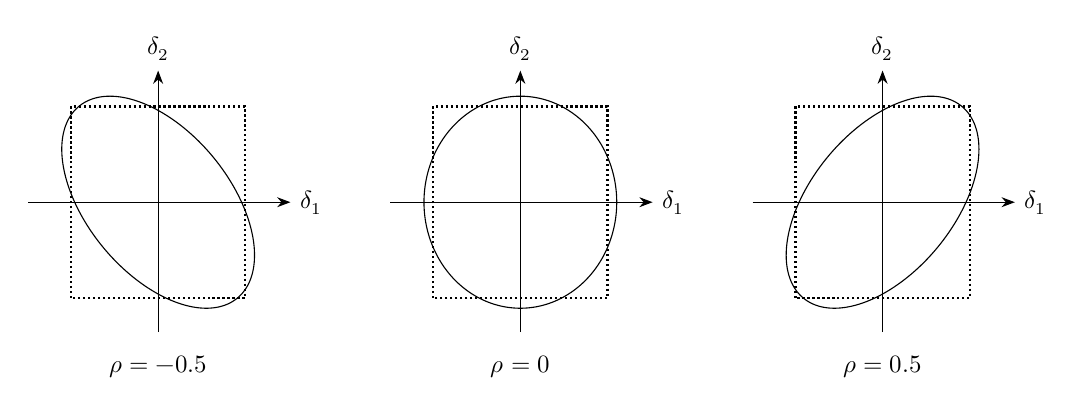
\begin{tikzpicture}[>=Stealth,font=\small]
 \foreach \corr/\shift in {-0.5/0,0/4.6,0.5/9.2}{
  \begin{scope}[xshift=\shift cm,x=1.5cm,y=1.1cm]
   \draw[->] (-1.1,0)--(1.12,0) node[right]{$\delta_1$};
   \draw[->] (0,-1.5)--(0,1.52) node[above]{$\delta_2$};
   \draw[densely dotted,thick] (-.737210,-1.105816) rectangle (.737210,1.105816);
   \draw[domain=0:360,samples=100,smooth,variable=\t]
   plot ({.816114*cos(\t)},
    {1.224171*(\corr*cos(\t)+sqrt(1-\corr*\corr)*sin(\t))});
   \node at (0,-1.9) {$\rho=\corr$};
  \end{scope}
 }
\end{tikzpicture}
\caption{Giữ phương sai thành phần, tâm và thang trục giống nhau:
 nét chấm Bonferroni không đổi; nét liền elip thay đổi theo tương quan.
 Các trục là độ lệch khỏi trung bình mẫu.}
\label{fig:rho_regions}
\end{figure}

\hieu{Hình chữ nhật trả lời ``mỗi trung bình có thể ở khoảng nào?''.
Elip còn trả lời ``hai trung bình có thể ở những vị trí ấy \emph{cùng
nhau} không?''. Với tương quan dương, cặp lệch cùng chiều được đánh giá
khác cặp lệch ngược chiều, dù từng độ lệch riêng có cùng độ lớn.}

Tuy nhiên, không suy rằng ``Bonferroni hoàn toàn không liên quan tương
quan''. Cần phân biệt ba điều:
\begin{enumerate}
 \item \textbf{Công thức biên của hình chữ nhật thành phần} không dùng
 hiệp phương sai chéo. Hình chữ nhật từ các khoảng thành phần $T^2$
 cũng có tính chất này nếu giữ đường chéo, $n,p,\alpha$ cố định.
 \item \textbf{Xác suất phủ đồng thời thực tế} có thể phụ thuộc tương
 quan vì các thống kê một chiều phụ thuộc nhau. Bonferroni chỉ bảo đảm
 một cận dưới, không khẳng định xác suất phủ bằng nhau trong mọi mô hình.
 \item \textbf{Khoảng cho tổ hợp} vẫn dùng $\mathbf a'S\mathbf a$.
 Với hiệu, $\Var$ mẫu là $s_{11}+s_{22}-2s_{12}$; tương quan dương
 làm khoảng hiệu hẹp hơn khi giữ các phương sai thành phần cố định.
\end{enumerate}

\paragraph{Nếu thêm một hiệu thì miền không còn đơn thuần chữ nhật.}
Khi danh sách có $\mu_1,\mu_2,\mu_1-\mu_2$, phải dùng $m=3$ cho
toàn bộ danh sách. Hai khoảng thành phần tạo hình chữ nhật rộng hơn
trường hợp $m=2$. Khoảng hiệu thêm điều kiện
\[
 |(\mu_1-\mu_2)-(\bar x_1-\bar x_2)|
 \le t_{n-1;1-\alpha/6}\sqrt{(s_{11}+s_{22}-2s_{12})/n}.
\]
Đó là một dải chéo; giao của dải với hình chữ nhật thường là đa giác.
Trong ví dụ hiện tại, điều kiện dải là $|\delta_1-\delta_2|\le1.0465$.
Không vẽ riêng hình chữ nhật rồi nói nó thể hiện đầy đủ cả ba khoảng.

\kiemtra{Giữ $s_{11},s_{22}$ và $n$ nhưng đổi dấu $s_{12}$:
 hình chữ nhật thành phần Bonferroni có đổi không? Không.
 Elip có đổi không? Có, hướng nghiêng đổi.
 Khoảng cho $\mu_1-\mu_2$ có đổi không? Có, vì có hạng $-2s_{12}$.}


\subsection{Khi nào Bonferroni hẹp hơn?}
Cho cùng một tổ hợp, cùng dữ liệu, cùng mức $\alpha$, tỉ số độ dài là
\begin{equation}
 \frac{\text{độ dài Bonferroni}}{\text{độ dài }T^2}
 =\frac{t_{n-1;1-\alpha/(2m)}}{\sqrt{c_T^2}}.
 \label{eq:widthratio}
\end{equation}
Chỉ khi tỉ số nhỏ hơn 1 mới nói Bonferroni hẹp hơn. Khi $m$ tăng, hệ số
Bonferroni tăng; do đó kết luận không đúng cho mọi danh sách hữu hạn.
Ví dụ với $n=100,p=2,\alpha=0.05$, hệ số $T^2$ khoảng 2.4983,
còn với $m=10000$, hệ số Bonferroni khoảng 4.8291.

Điều quan trọng không chỉ là độ rộng: phải chọn bảo đảm phù hợp câu hỏi.
Nếu chỉ có vài phát biểu xác định trước, Bonferroni dễ áp dụng.
Nếu cần mọi hướng hoặc chọn hướng sau khi xem dữ liệu, $T^2$ phù hợp hơn.
Không tính nhiều khoảng rồi chỉ giữ những khoảng ``đẹp'' mà coi $m$ là
số khoảng cuối cùng đã chọn.

\kiemtra{Các khoảng Bonferroni có cần độc lập không? Không.
Nếu có 4 trung bình và 1 hiệu cần báo cáo thì $m=5$, không phải 4.}

\clearpage
\section{Suy diễn mẫu lớn và cách chọn phương pháp}
\label{sec:large}

\subsection{Điểm thay đổi: phân phối giới hạn thay cho phân phối chính xác}
Trong tổng thể không chuẩn, $T^2$ vẫn tính được nếu $S$ khả nghịch,
nhưng công thức $F$ của mẫu chuẩn không còn là một kết quả chính xác.
Với mẫu iid, $p$ cố định, trung bình và hiệp phương sai hữu hạn, $\Sigma$
xác định dương, Phần~\ref{sec:sampling} đã cho
\[
 n(\Xbar-\vmu)'S^{-1}(\Xbar-\vmu)\xrightarrow{d}\chi^2_p.
\]
Suy diễn mẫu lớn dùng phân phối giới hạn này để xấp xỉ ngưỡng.
\nguon{Chương 4, §4.5, (4-28), tr.~176; Chương 5, §5.5, (5-31), tr.~235}

\begin{result}[Kiểm định xấp xỉ]
Với các điều kiện trên và $n$ đủ lớn, bác bỏ $H_0:\vmu=\vmu_0$ ở mức
xấp xỉ $\alpha$ khi
\begin{equation}
 T^2=n(\xbar-\vmu_0)'S^{-1}(\xbar-\vmu_0)>\chi^2_{p;1-\alpha}.
 \label{eq:largetest}
\end{equation}
Giá trị p xấp xỉ là đuôi phải của $\chi^2_p$ tại $T^2$ quan sát.
\end{result}
\nguon{Chương 5, §5.5, Result 5.4, tr.~235}

Thống kê không đổi, nhưng ngưỡng thay đổi. Nếu tổng thể chuẩn và có đủ
điều kiện, có thể tiếp tục dùng ngưỡng $F$ chính xác dù mẫu lớn.
Không bắt buộc bỏ kết quả chính xác để dùng xấp xỉ.

\subsection{Khoảng tin cậy xấp xỉ}
Miền cho trung bình dùng
\[
 n(\xbar-\vmu)'S^{-1}(\xbar-\vmu)\le\chi^2_{p;1-\alpha}.
\]
Tương ứng, các khoảng đồng thời cho mọi tổ hợp là
\begin{equation}
 \mathbf a'\xbar\pm\sqrt{\chi^2_{p;1-\alpha}}
 \sqrt{\frac{\mathbf a'S\mathbf a}{n}}.
 \label{eq:largeinterval}
\end{equation}
Với từng thành phần, đặt $\mathbf a=\mathbf e_i$; với hiệu hai thành
phần, đặt $\mathbf a=\mathbf e_i-\mathbf e_k$ như trước.
\nguon{Chương 5, §5.5, Result 5.5, tr.~235--236}

Cho $m$ tổ hợp xác định trước, Bonferroni mẫu lớn dùng
\begin{equation}
 \mathbf a_j'\xbar\pm z_{1-\alpha/(2m)}
 \sqrt{\frac{\mathbf a_j'S\mathbf a_j}{n}},\qquad j=1,\ldots,m.
 \label{eq:largebonf}
\end{equation}
Đây là hệ quả của CLT một chiều cho từng tổ hợp và bất đẳng thức hợp.
$z_\gamma$ là phân vị của $\N(0,1)$.
Trong tổng thể không chuẩn, việc giữ hệ số $t$ không tự làm bảo đảm trở
thành chính xác; cả cách dùng $t$ lẫn $z$ đều cần đánh giá xấp xỉ.

\subsection{Một ví dụ để thấy độ chênh giữa hai ngưỡng}
\begin{example}[Số tóm tắt giả định, $n=100$]
Giả sử $p=2$, $n=100$, $\xbar=(6,10)'$ và
$S=\begin{pmatrix}8&-10/3\\-10/3&2\end{pmatrix}$.
Đây là một mẫu giả định mới; không lấy bốn quan sát rồi tự đổi $n$ thành 100.
Kiểm định $\vmu_0=(7,11)'$ cho
\[
 T^2=100\frac{75}{22}=340.9091.
\]
Ngưỡng chi-bình phương 95\% là 5.9915; nếu mẫu chuẩn, ngưỡng $F$ chính
xác là
\[
 \frac{2\cdot99}{98}F_{2,98;0.95}\approx6.2415.
\]
Cả hai cách đều bác bỏ ở ví dụ này.
Các khoảng thành phần chi-bình phương là
\[
 \mu_1:6\pm0.6923,\qquad\mu_2:10\pm0.3462.
\]
Với $m=3$ phát biểu định trước, hệ số Bonferroni chuẩn là
$z_{1-0.05/6}\approx2.3940$.
\end{example}

Hãy so với mẫu $n=4$ ở phần Hotelling: trung bình và $S$ có thể giống nhau,
nhưng sai số chuẩn của trung bình và ngưỡng suy diễn khác nhau. Vì vậy
không thể diễn giải độ chắc chắn mà quên kích thước mẫu.

\subsection{``Mẫu lớn'' không có một ngưỡng đúng cho mọi dữ liệu}
Một quy tắc thực hành thường gặp là $n-p\ge30$. Nó có thể hữu ích cho
ôn tập hoặc chỉ dẫn sơ bộ, nhưng không phải giả thiết của CLT hay Slutsky,
và không bảo đảm xấp xỉ tốt cho mọi phân phối.
Sách thảo luận rằng độ chính xác còn phụ thuộc số chiều và dạng phân phối;
hai bài toán cùng $n-p$ vẫn có thể khác nhau nhiều.
\nguon{Chương 5, §5.5, thảo luận về kích thước mẫu và lệch chuẩn, tr.~236}

Các yếu tố cần xem gồm độ lệch, đuôi nặng, ngoại lệ, sự phụ thuộc giữa
quan sát, tỉ lệ giữa $p$ và $n$, và tình trạng gần suy biến của $S$.
Giới hạn với $p$ cố định không tự áp dụng khi $p$ tăng nhanh cùng $n$.
Nếu phương sai không hữu hạn hoặc dữ liệu phụ thuộc thời gian, các công
thức giới hạn trong bài giảng không tự được bảo đảm.

\luuy{Mẫu lớn giúp trung bình mẫu gần chuẩn; nó không sửa được sai
thiết kế lấy mẫu, không làm quan sát phụ thuộc trở thành iid, và không
biến ma trận gần suy biến thành một ước lượng tốt.}

\subsection{Kiểm tra mô hình trước khi suy diễn}
Đối với dữ liệu thực, nên kiểm tra:
\begin{enumerate}
 \item \textbf{Thiết kế mẫu:} các hàng có phải những đối tượng độc lập,
 cùng cơ chế lấy mẫu hay có đo lặp, chuỗi thời gian, phân cụm?
 \item \textbf{Chất lượng dữ liệu:} đơn vị, giá trị thiếu, cột hằng,
 biến trùng và phép biến đổi đã dùng.
 \item \textbf{Đồ thị:} histogram, Q--Q plot cho từng biến; scatter plot
 cho các cặp; điểm ngoại lệ và các dạng phi tuyến.
 \item \textbf{Hiệp phương sai:} $n>p$, hạng và mức độ gần suy biến.
\end{enumerate}
Các Q--Q plot biên nhìn đẹp không chứng minh chuẩn đồng thời, như phản
ví dụ ở Phần~\ref{sec:linear}. Đồ thị là công cụ đánh giá, không thay thế
toàn bộ giả thiết. Khi đã biến đổi dữ liệu, kết luận thường nói về trung
bình \emph{trên thang biến đổi}; ví dụ $\E(\log X)$ không bằng
$\log\E(X)$ nói chung.
\nguon{Chương 4, §4.6, tr.~177--186; §4.7, tr.~187--192; biến đổi dữ liệu ở §4.8, từ tr.~192}

Không tự xóa ngoại lệ chỉ để đạt kết quả mong muốn. Cần xác định đó là
lỗi nhập liệu hay quan sát có ý nghĩa, rồi nêu rõ xử lý. Nếu cần phương
pháp cho dữ liệu phụ thuộc, hiệp phương sai suy biến hoặc cao chiều, phải
xây dựng mô hình khác; chúng nằm ngoài phạm vi bài giảng này.

\subsection{Bảng chọn phương pháp}
\begin{center}
\small
\begin{tabular}{p{.30\linewidth}p{.30\linewidth}p{.31\linewidth}}
\toprule
Câu hỏi & Điều kiện chính & Công cụ\\
\midrule
Phân phối một tổ hợp hoặc vectơ con & Vectơ gốc chuẩn & $A\vmu$, $A\Sigma A'$; chọn khối\\
Phân phối khi biết một khối & Chuẩn chung, khối đã biết khả nghịch & Công thức có điều kiện\\
Độc lập giữa các tổ hợp & Chuẩn đồng thời & Kiểm tra $\mathbf a'\Sigma\mathbf b=0$\\
Kiểm định vectơ trung bình chính xác & Mẫu iid chuẩn, $n>p$, $\Sigma$ xác định dương & $T^2$ và ngưỡng $F$\\
Mọi tổ hợp của trung bình & Như trên & Khoảng đồng thời $T^2$\\
Ít tổ hợp định trước & Mẫu iid chuẩn & Bonferroni với $m$ phát biểu\\
Trung bình, tổng thể không chuẩn & Iid, moment hữu hạn, $p$ cố định, mẫu đủ lớn & Ngưỡng $\chi^2$; Bonferroni $z$\\
\bottomrule
\end{tabular}
\end{center}

\subsection{Liên hệ với BTVN 1--2}
\begin{center}
\small
\begin{tabular}{lp{.68\linewidth}}
\toprule
Bài & Phần cần đọc và thao tác chính\\
\midrule
2.1 & Phần 3: chọn vectơ trung bình và ma trận hiệp phương sai con.\\
2.2 & Phần 3: kiểm tra khối hiệp phương sai hoặc hiệp phương sai của tổ hợp.\\
2.3 & Phần 4: phân hoạch theo biến mục tiêu và biến đã biết.\\
2.4a,b & Phần 3: tổ hợp tuyến tính; phương trình triệt tiêu hiệp phương sai.\\
2.9a--d & Phần 5 và 8: phân phối trung bình mẫu, $T^2$ và xấp xỉ; chọn theo giả thiết của từng câu.\\
3.1 & Phần 6: tính $T^2$, đổi sang $F$, so ngưỡng và kết luận.\\
3.2 & Phần 6: biến đổi đồng bộ dữ liệu, $S$ và trung bình giả thuyết.\\
3.3--3.5 & Phần 7: bảo đảm đồng thời, miền elip, khoảng thành phần và các hiệu; đếm đúng $m$.\\
3.6a--d & Phần 8: suy diễn mẫu lớn, khoảng $\chi^2$ và Bonferroni; nhớ hạng hiệp phương sai.\\
\bottomrule
\end{tabular}
\end{center}
Số bài ở đây theo BTVN địa phương. Chúng không phải số Result hay số
Exercise trong giáo trình. Khi đối chiếu lời giải, phải dùng đúng bộ dữ
kiện của từng bài; không suy rằng cùng một ký hiệu $\Sigma$ nghĩa là cùng
một ma trận ở mọi trang.

\kiemtra{Nếu tổng thể chuẩn và $n=100$, có bắt buộc dùng ngưỡng
$\chi^2$ không? Không. Ngưỡng $F$ chính xác vẫn dùng được.}

\clearpage
\section{Tự luyện: từ đọc tham số đến chọn phương pháp}
\label{sec:practice}
Các bài dưới đây được biên soạn để luyện theo bài giảng. Khi làm, ghi cả
giả thiết và diễn giải kết quả, không chỉ viết một con số. Đáp án ở
Phụ lục~\ref{app:answers}; nên làm xong mỗi nhóm rồi mới đối chiếu.

\subsection{Nhóm A: tham số, tổ hợp và điều kiện}
\begin{enumerate}[label=\textbf{Bài \arabic*.},ref=\arabic*,series=practice]
\item Cho $\vmu=(10,20)'$,
$\Sigma=\begin{pmatrix}4&2\\2&9\end{pmatrix}$.
Hãy đọc trung bình, độ lệch chuẩn và tương quan; kiểm tra xác định dương;
tính $\Sigma^{-1}$. Vì sao chỉ biết hai phương sai chưa đủ để xác định
phân phối chuẩn hai chiều?

\item Với $\mathbf X\sim\N_3(\vmu,\Sigma)$ theo
\eqref{eq:running3d}, tìm phân phối của $(X_3,X_1)'$ và của $X_2$.
Viết ma trận chọn cho vectơ con. Giải thích vì sao không dùng công thức
có điều kiện ở đây.

\item Vẫn dùng \eqref{eq:running3d}, đặt $Y=X_1+2X_2-X_3$.
Tìm phân phối $Y$ bằng hai cách tính phương sai: nhân ma trận và khai triển
hiệp phương sai. Giải thích dấu của hạng chứa $\Cov(X_1,X_3)$.

\item Đặt $U=X_1+X_3$, $V=X_1-X_3$ trong cùng mô hình.
$U,V$ có độc lập không? $X_2,U$ có độc lập không? Nếu thay yêu cầu thứ
nhất bằng ``tìm $c$ sao cho $X_1+cX_3$ độc lập với $X_1-X_3$'', nghiệm là gì?

\item Cho $Z\sim\N(0,1)$ và $W=Z^2$.
Tính $\Cov(Z,W)$ và giải thích vì sao không suy ra độc lập.
Một người nói ``chỉ cần mỗi biến riêng chuẩn thì không tương quan tương
đương độc lập''. Hãy dùng phản ví dụ ở Phần~\ref{sec:linear} để bác bỏ.

\item Tìm phân phối $(X_1,X_2)'\mid X_3=4$ trong
\eqref{eq:running3d}. Viết đủ bốn khối hiệp phương sai cần dùng.
So sánh với phân phối biên và giải thích biến nào được cập nhật.
\end{enumerate}

\subsection{Nhóm B: phân phối mẫu và Hotelling}
\begin{enumerate}[label=\textbf{Bài \arabic*.},ref=\arabic*,resume=practice]
\item Mẫu iid $\N_2((10,20)',\begin{pmatrix}4&3\\3&9\end{pmatrix})$
có $n=25$. Nêu phân phối của $\Xbar$, phân phối của $24S$ và mối quan
hệ độc lập. So sánh độ lệch chuẩn của $X_{j1}$ và $\bar X_1$.
Nếu tổng thể không chuẩn nhưng vẫn có các moment hữu hạn, kết quả nào
về moment còn đúng và kết quả phân phối nào không còn chính xác?

\item Mẫu iid chuẩn có dữ liệu
\[
 \mathbf D=\begin{pmatrix}1&2\\2&1\\3&4\\4&3\\5&5\end{pmatrix}.
\]
Tính $\xbar,S,S^{-1}$; kiểm định $\vmu_0=(2,2)'$ mức 5\%.
Cho $F_{2,3;0.95}\approx9.5521$.
Tính thống kê có phân phối $F$ và viết kết luận bằng lời.
Viết log-hợp lý của mẫu; dùng phân rã tổng tích ngoài để tìm MLE trung
bình, rồi tìm MLE hiệp phương sai và so sánh với $S$.

\item Dùng mẫu Bài 8. Đặt
$C=\diag(100,0.1)$, $\mathbf d=(5,-2)'$.
Tính trung bình, hiệp phương sai và vectơ giả thuyết sau biến đổi.
Kiểm tra $T^2$ không đổi. Nếu bảng dữ liệu viết mỗi quan sát thành hàng,
phải nhân bảng với $C$ hay $C'$ trong công thức tổng quát?
Giải thích vì sao giá trị p và quyết định kiểm định cũng không đổi;
đẳng thức bất biến có cần giả thiết chuẩn không?
\end{enumerate}

\subsection{Nhóm C: khoảng đồng thời, hợp lý và mẫu lớn}
\begin{enumerate}[label=\textbf{Bài \arabic*.},ref=\arabic*,resume=practice]
\item Với số tóm tắt $n=40$ ở \eqref{eq:intervaldata}, cần báo cáo
$\mu_1,\mu_2,\mu_1-\mu_2,2\mu_1-\mu_2$.
Xác định $m$, tính ước lượng và sai số chuẩn của tổ hợp cuối.
Lập khoảng $T^2$ và Bonferroni cho tổ hợp đó.
Cho $t_{39;1-0.05/8}\approx2.6189$.
Có được dùng hệ số Bonferroni tính với $m=3$ cho cả bốn phát biểu không?
Xét riêng bài toán \emph{chỉ báo cáo hai trung bình}, dùng $m=2$ và
$t_{39;0.9875}\approx2.3313$. Dựng hình chữ nhật Bonferroni và kiểm tra
hai điểm $P=(10.70,18.95)'$, $R=(10.80,20.60)'$ trong chữ nhật và elip.
Nếu đổi $s_{12}$ từ 3 thành $-3$, miền nào đổi, và sai số chuẩn của
$2\mu_1-\mu_2$ tăng hay giảm?

\item Dùng Bài 8, tính $\widehat\Sigma$ và
$\widehat\Sigma_0$ dưới giả thuyết $(2,2)'$.
Từ định thức, tính $\lambda_W$, $\Lambda_{\mathrm{LR}}$ và $T^2$.
Vì sao Wilks' lambda không phải luôn là giá trị p?

\item Một mẫu iid từ tổng thể không chuẩn, có moment bậc hai hữu hạn,
cho $n=100,p=2$, $\xbar=(0.2,0.1)'$, $S=I_2$.
Với $H_0:\vmu=0$, tính kiểm định chi-bình phương xấp xỉ mức 5\% và
khoảng thành phần đồng thời chi-bình phương. Cho
$\chi^2_{2;0.95}=5.9915$, $z_{0.9875}=2.2414$.
Tính thêm khoảng Bonferroni cho hai thành phần.
Sau đó đánh giá hai phát biểu: ``$n=20,p=25$ vẫn dùng $S^{-1}$ bình thường'';
``$n=2000,p=1900$ đủ điều kiện xấp xỉ chỉ vì $n-p=100$''.
\end{enumerate}

\subsection{Tự đánh giá trước khi xem đáp án}
Bạn đã nắm ý chính khi có thể trả lời bằng lời:
\begin{itemize}
 \item Vì sao $\Sigma$ và $\Sigma/n$ xuất hiện trong hai bài toán khác nhau?
 \item Khi nào biết một biến khác giúp giảm phương sai có điều kiện?
 \item Tại sao $T^2$ có hệ số $n$ và phải chuyển đổi trước khi so với $F$?
 \item Miền elip khác hình chữ nhật từ khoảng thành phần như thế nào?
 \item Bonferroni bảo vệ danh sách nào, và ai quyết định số $m$?
 \item Chuẩn của trung bình mẫu có nghĩa là các quan sát gốc chuẩn không?
\end{itemize}
Nếu tính được số nhưng chưa giải thích được các câu này, hãy đọc lại phần
``Hiểu bằng lời'' tương ứng. Mục tiêu là chọn đúng công cụ cho câu hỏi,
không phải chỉ nhận ra hình dáng của một công thức.

\appendix
\clearpage
\section{Chứng minh đọc sâu}
\label{sec:proofs}
Phần này có thể đọc ở lượt thứ hai. Các chứng minh làm rõ vì sao công
thức có dạng như trong mạch chính; không cần thuộc lòng từng dòng để bắt
đầu giải bài. Những định lý nền như CLT và phân phối Hotelling được dùng
như kết quả đã có trong giáo trình, không tuyên bố chứng minh đầy đủ ở đây.

\subsection{Làm trắng và phân phối khoảng cách}
\label{app:whitening}
Vì $\Sigma$ đối xứng xác định dương, tồn tại phân rã phổ
\[
 \Sigma=QDQ',\qquad Q'Q=I,
 \quad D=\diag(\lambda_1,\ldots,\lambda_p),\quad\lambda_i>0.
\]
Đặt $\Sigma^{-1/2}=QD^{-1/2}Q'$ và
$\mathbf Z=\Sigma^{-1/2}(\mathbf X-\vmu)$.
Theo tính chất biến đổi tuyến tính,
\[
 \mathbf Z\sim\N_p(0,\Sigma^{-1/2}\Sigma\Sigma^{-1/2})=\N_p(0,I).
\]
Các thành phần của $\mathbf Z$ chuẩn đồng thời và không tương quan, nên
độc lập. Mặt khác,
\[
 (\mathbf X-\vmu)'\Sigma^{-1}(\mathbf X-\vmu)
 =\mathbf Z'\mathbf Z=\sum_{i=1}^p Z_i^2\sim\chi^2_p.
\]
Đây là chứng minh Result 4.7(a). Việc lấy phân vị của phân phối vừa tìm
cho ngay kết luận về xác suất của elipsoid.
\nguon{Chương 4, §4.2, Result 4.7 và chứng minh, tr.~163--164}

\subsection{Phân phối có điều kiện qua phần dư}
Đặt $B=\Sigma_{12}\Sigma_{22}^{-1}$ và
\[
 \mathbf R=\mathbf X_1-\vmu_1-B(\mathbf X_2-\vmu_2).
\]
Vectơ $(\mathbf R',\mathbf X_2')'$ chuẩn vì là biến đổi tuyến tính của
vectơ gốc. Ta tính
\[
 \Cov(\mathbf R,\mathbf X_2)=\Sigma_{12}-B\Sigma_{22}=0.
\]
Do đó $\mathbf R$ độc lập với $\mathbf X_2$.
Hiệp phương sai phần dư là
\begin{align*}
 \Cov(\mathbf R)
 &=\Sigma_{11}-B\Sigma_{21}-\Sigma_{12}B'+B\Sigma_{22}B'\\
 &=\Sigma_{11}-\Sigma_{12}\Sigma_{22}^{-1}\Sigma_{21}.
\end{align*}
Ở dòng cuối ta dùng tính đối xứng của $\Sigma_{22}$.
Khi biết $\mathbf X_2=\mathbf x_2$,
\[
 \mathbf X_1=\vmu_1+B(\mathbf x_2-\vmu_2)+\mathbf R.
\]
Phần trước $\mathbf R$ là hằng số có điều kiện, còn $\mathbf R$ vẫn giữ
nguyên phân phối. Suy ra cả trung bình và hiệp phương sai trong
\eqref{eq:conditionalmean}--\eqref{eq:conditionalcov}.
\nguon{Chương 4, §4.2, chứng minh Result 4.6, tr.~161}

Hiệp phương sai được giảm theo nghĩa ma trận:
\[
 \Sigma_{11}-\Sigma_{11\mid2}
 =\Sigma_{12}\Sigma_{22}^{-1}\Sigma_{21}\succeq0.
\]
Thật vậy với mọi $\mathbf a$,
$\mathbf a'\Sigma_{12}\Sigma_{22}^{-1}\Sigma_{21}\mathbf a\ge0$.
Do đó phương sai của \emph{bất kỳ tổ hợp tuyến tính} của khối mục tiêu
không tăng khi điều kiện hóa trong mô hình chuẩn này. ``Giảm theo nghĩa
ma trận'' không có nghĩa mọi phần tử hiệp phương sai đều giảm về mặt số học.

\subsection{Vì sao trung bình mẫu độc lập với \texorpdfstring{$S$}{S}?}
\label{app:wishart}
Viết bảng quan sát thành ma trận $D$ kích thước $n\times p$.
Chọn ma trận trực giao $H$ kích thước $n\times n$, có hàng đầu
$\mathbf 1'/\sqrt n$, các hàng còn lại vuông góc với $\mathbf1$.
Đặt $Y=HD$, với các hàng được xem là vectơ quan sát mới.

Hàng đầu là $\sqrt n\Xbar'$ và có trung bình $\sqrt n\vmu'$.
Các hàng còn lại có trung bình 0. Hiệp phương sai giữa hàng $r$ và hàng
$s$ của $Y$ là
\[
 \sum_{j=1}^n H_{rj}H_{sj}\Sigma
 =\begin{cases}\Sigma,&r=s,\\0,&r\ne s.\end{cases}
\]
Các hàng chuẩn đồng thời, nên độc lập. Viết $\mathbf Y_r$ là chuyển vị
của hàng $r$, ta có $\mathbf Y_2,\ldots,\mathbf Y_n$ iid $\N_p(0,\Sigma)$.
Tính trực giao cho
\[
 (n-1)S=D'\left(I_n-\frac{\mathbf1\mathbf1'}n\right)D
 =\sum_{r=2}^n\mathbf Y_r\mathbf Y_r'.
\]
Vế phải là Wishart với $n-1$ bậc tự do, chỉ phụ thuộc các hàng 2 đến $n$.
Hàng đầu quyết định trung bình mẫu và độc lập với những hàng đó, nên
$\Xbar\perp S$.
\nguon{Khai triển bổ sung cho kết quả phân phối mẫu (4-23), Chương 4, §4.4, tr.~174}

\subsection{Kiểm tra cực đại MLE bằng trị riêng}
\label{app:mle_global}
Nếu muốn tránh đạo hàm ma trận ở Phần~\ref{sec:mle_derivation}, có thể
kiểm tra cực đại toàn cục bằng bất đẳng thức một biến.
Đặt $M=A/n\succ0$ và $B=M^{1/2}\Sigma^{-1}M^{1/2}\succ0$.
Gọi $\lambda_1,\ldots,\lambda_p$ là các trị riêng của $B$.
Từ log-hợp lý đã đặt $\vmu=\xbar$, ta có
\begin{align*}
 \ell(\xbar,\Sigma)-\ell(\xbar,M)
 &=\frac n2\bigl[\log|B|-\tr(B)+p\bigr]\\
 &=\frac n2\sum_{i=1}^p(\log\lambda_i-\lambda_i+1)\le0.
\end{align*}
Dòng cuối dùng $\log u\le u-1$ với $u>0$, dấu bằng chỉ khi $u=1$.
Cực đại đạt duy nhất khi mọi $\lambda_i=1$, tức $B=I$ vì $B$ đối xứng,
và do đó $\Sigma=M=A/n$. Bước tìm trung bình đã bảo đảm
$\ell(\vmu,\Sigma)\le\ell(\xbar,\Sigma)$, nên đây là cực đại đồng thời.
\nguon{Lập luận tương đương Chương 4, §4.3, Result 4.10, tr.~170--171,
 và Result 4.11, tr.~171--172}

Nếu $A$ có hạng $r<p$, viết
$A=U\diag(a_1,\ldots,a_r,0,\ldots,0)U'$ với $a_i>0$.
Chọn
\[
 \Sigma_\varepsilon=U\diag(a_1/n,\ldots,a_r/n,
 \varepsilon,\ldots,\varepsilon)U',\qquad\varepsilon>0.
\]
Khi đó $\tr(\Sigma_\varepsilon^{-1}A)=nr$ không đổi, nhưng
$\log|\Sigma_\varepsilon|=\text{hằng số}+(p-r)\log\varepsilon
\to-\infty$ khi $\varepsilon\downarrow0$.
Suy ra $\ell(\xbar,\Sigma_\varepsilon)\to+\infty$.
Không có cực đại hữu hạn trong miền hiệp phương sai xác định dương;
ma trận suy biến $A/n$ không khắc phục vấn đề bằng cách được gọi là
nghiệm trong mô hình không suy biến.

Chứng minh bất biến của $T^2$, gồm cả giá trị p và quyết định kiểm định,
được trình bày ngay trong Phần~\ref{sec:invariance_proof} để thuận tiện
đọc cùng ví dụ. Không cần lặp lại chứng minh đó ở đây.

\subsection{Tỷ số định thức và Wilks' lambda}
Đặt $A=(n-1)S$ và $\mathbf r=\xbar-\vmu_0$. Tách tổng bình phương quanh
giá trị giả thuyết:
\begin{align*}
 \sum_j(\mathbf x_j-\vmu_0)(\mathbf x_j-\vmu_0)'
 &=\sum_j\bigl[(\mathbf x_j-\xbar)+\mathbf r\bigr]
 \bigl[(\mathbf x_j-\xbar)+\mathbf r\bigr]'\\
 &=A+n\mathbf r\mathbf r'.
\end{align*}
Hai hạng chéo bằng 0 vì $\sum_j(\mathbf x_j-\xbar)=0$.
Bổ đề định thức cho cập nhật hạng một là
\[
 |A+\mathbf u\mathbf v'|=|A|(1+\mathbf v'A^{-1}\mathbf u).
\]
Lấy $\mathbf u=n\mathbf r$, $\mathbf v=\mathbf r$:
\[
 \frac{|A+n\mathbf r\mathbf r'|}{|A|}
 =1+n\mathbf r'A^{-1}\mathbf r=1+\frac{T^2}{n-1}.
\]
Vì $n\widehat\Sigma=A$ và $n\widehat\Sigma_0=A+n\mathbf r\mathbf r'$,
ta có
\[
 \frac{|\widehat\Sigma|}{|\widehat\Sigma_0|}
 =\left(1+\frac{T^2}{n-1}\right)^{-1}.
\]
Để hoàn tất kết nối với hợp lý, ở MLE của mô hình chuẩn, phần mũ của hàm
hợp lý bằng $e^{-np/2}$ ở cả hai mô hình. Hệ số $(2\pi)^{-np/2}$ cũng
giống nhau, nên tỷ số cực đại chỉ còn
$\Lambda_{\mathrm{LR}}=(|\widehat\Sigma|/|\widehat\Sigma_0|)^{n/2}$.
\nguon{Chương 5, §5.3, chứng minh Result 5.1, tr.~218; phân rã tổng bình phương (4-14), tr.~169}

\subsection{Hình chiếu elipsoid và khoảng đồng thời}
\label{app:projection}
Cho $\mathbf h=\vmu-\xbar$. Nếu $\vmu\in\mathcal C$, thì
$\mathbf h'S^{-1}\mathbf h\le c_T^2/n$.
Viết
\[
 \mathbf a'\mathbf h=(S^{1/2}\mathbf a)'(S^{-1/2}\mathbf h).
\]
Bất đẳng thức Cauchy--Schwarz cho
\begin{align*}
 |\mathbf a'\mathbf h|
 &\le\sqrt{\mathbf a'S\mathbf a}
 \sqrt{\mathbf h'S^{-1}\mathbf h}\\
 &\le\sqrt{c_T^2}\sqrt{\mathbf a'S\mathbf a/n}.
\end{align*}
Đây chính là hai đầu khoảng \eqref{eq:t2interval}. Với $\mathbf a\ne0$,
dấu bằng đạt tại
\[
 \mathbf h=\pm\sqrt{\frac{c_T^2}{n}}
 \frac{S\mathbf a}{\sqrt{\mathbf a'S\mathbf a}}.
\]
Vì thế khoảng là hình chiếu \emph{chính xác} của elipsoid, không phải
một xấp xỉ về hình học.

Theo chiều ngược lại, nếu khoảng phủ cho mọi $\mathbf a$, chọn
$\mathbf a=S^{-1}\mathbf h$ để suy ra
$\mathbf h'S^{-1}\mathbf h\le c_T^2/n$ (trường hợp $\mathbf h=0$ hiển nhiên).
Do đó biến cố ``mọi khoảng đều phủ'' tương đương ``elipsoid phủ vectơ
trung bình'', có xác suất $1-\alpha$ dưới mô hình chuẩn.
\nguon{Chương 5, §5.4, (5-23) và Result 5.3, tr.~225; Supplement 5A về hình chiếu}

\subsection{Bonferroni và Slutsky: hai kiểu bảo đảm khác nhau}
Cho $C_j$ là biến cố khoảng thứ $j$ phủ đúng. Với mọi kết quả ngẫu nhiên,
\[
 \mathbf1_{\cup_j C_j^c}\le\sum_j\mathbf1_{C_j^c}.
\]
Lấy kỳ vọng và phần bù:
\[
 \Prob\left(\bigcap_j C_j\right)
 =1-\Prob\left(\bigcup_j C_j^c\right)
 \ge1-\sum_j\Prob(C_j^c).
\]
Nếu mỗi khoảng có xác suất sai $\alpha/m$, cả nhóm có xác suất phủ
ít nhất $1-\alpha$. Bất đẳng thức luôn đúng; việc xác suất sai của từng
khoảng có \emph{đúng} bằng $\alpha/m$ hay chỉ xấp xỉ tùy vào phương pháp
dựng khoảng và mô hình.
\nguon{Chương 5, §5.4, (5-28), tr.~232}

Với Slutsky, đặt $\mathbf Z_n=\sqrt n(\Xbar-\vmu)$.
CLT cho $\mathbf Z_n\xrightarrow{d}\mathbf Z\sim\N_p(0,\Sigma)$.
Luật số lớn và tính liên tục của phép nghịch đảo tại ma trận xác định
dương cho $S^{-1}\xrightarrow{P}\Sigma^{-1}$.
Slutsky và phép ánh xạ liên tục dẫn đến
\[
 \mathbf Z_n'S^{-1}\mathbf Z_n\xrightarrow{d}
 \mathbf Z'\Sigma^{-1}\mathbf Z\sim\chi^2_p.
\]
Không cần $\Xbar$ và $S$ độc lập ở mẫu hữu hạn cho lập luận giới hạn này.
Đây là một lý do suy diễn mẫu lớn có thể vượt ra ngoài tổng thể chuẩn.
\nguon{Diễn giải bổ sung cho Chương 4, §4.5, (4-28), tr.~176}

\clearpage
\section{Đáp án và lời giải ngắn cho bài tự luyện}
\label{app:answers}
\subsection*{Bài 1--3: đọc tham số và biến đổi}
\noindent\textbf{Bài 1.}
Trung bình là 10 và 20; độ lệch chuẩn là 2 và 3; tương quan
$2/(2\cdot3)=1/3$. $|\Sigma|=36-4=32>0$, $\sigma_{11}>0$, nên
xác định dương. Nghịch đảo là
$\frac1{32}\begin{pmatrix}9&-2\\-2&4\end{pmatrix}$.
Các phương sai không cho biết hiệp phương sai ngoài đường chéo; thiếu
nó, hướng và độ dài các trục elip chưa được xác định.

\noindent\textbf{Bài 2.}
Ma trận chọn $A=\begin{pmatrix}0&0&1\\1&0&0\end{pmatrix}$, nên
\[
 (X_3,X_1)'\sim\N_2\left((2,1)',
 \begin{pmatrix}2&-1\\-1&4\end{pmatrix}\right),\qquad
 X_2\sim\N(-1,5).
\]
Không biết giá trị biến nào khác, nên đây là phân phối biên.

\noindent\textbf{Bài 3.}
$\mathbf a=(1,2,-1)'$, $\mathbf a'\vmu=-3$ và
$\Sigma\mathbf a=(5,10,-3)'$, do đó phương sai $5+20+3=28$.
Cách khai triển: $4+4\cdot5+2+2(1)(-1)(-1)=28$.
Hạng chéo là dương vì hệ số của $X_3$ âm và hiệp phương sai với $X_1$
cũng âm. Vậy $Y\sim\N(-3,28)$.

\subsection*{Bài 4--6: độc lập và điều kiện}
\noindent\textbf{Bài 4.}
$\Cov(U,V)=\Var(X_1)-\Var(X_3)=2\ne0$: không độc lập.
$\Cov(X_2,U)=0+0=0$: độc lập nhờ chuẩn đồng thời.
Với $U_c=X_1+cX_3$,
\[
 \Cov(U_c,V)=4-(-1)+c(-1-2)=5-3c.
\]
Nghiệm $c=5/3$.

\noindent\textbf{Bài 5.}
$\Cov(Z,Z^2)=\E(Z^3)=0$, nhưng $Z^2$ được xác định bởi $Z$, nên phụ
thuộc. Để minh họa chuẩn của từng biên vẫn chưa đủ, dùng $V=BZ$ với $B$
độc lập và nhận $\pm1$ đồng xác suất. Hai biên chuẩn, hiệp phương sai
0, nhưng $|V|=|Z|$; chúng không chuẩn đồng thời và không độc lập.

\noindent\textbf{Bài 6.}
Khối mục tiêu $\mathbf U=(X_1,X_2)'$ có
$\vmu_U=(1,-1)'$, $\Sigma_{UU}=\diag(4,5)$.
Khối đã biết là $V=X_3$, $\mu_V=2$, $\Sigma_{VV}=2$;
$\Sigma_{UV}=(-1,0)'$, $\Sigma_{VU}=(-1,0)$.
\[
 \mathbf U\mid V=4\sim\N_2\left((0,-1)',\diag(7/2,5)\right).
\]
Chỉ thành phần thứ nhất được cập nhật; $X_2$ độc lập với $X_3$.
Trong phân phối có điều kiện này, hai thành phần vẫn độc lập vì ma trận
hiệp phương sai chéo bằng không và chúng chuẩn đồng thời.

\subsection*{Bài 7--9: phân phối mẫu và kiểm định}
\noindent\textbf{Bài 7.}
\[
 \Xbar\sim\N_2\left((10,20)',
 \begin{pmatrix}.16&.12\\.12&.36\end{pmatrix}\right),\qquad
 24S\sim W_{2,24}(\Sigma),\quad\Xbar\perp S.
\]
Độ lệch chuẩn của $X_{j1}$ là 2, của $\bar X_1$ là 0.4.
Với mẫu iid không chuẩn, $\E(\Xbar)=\vmu$, $\Cov(\Xbar)=\Sigma/25$
và $\E(S)=\Sigma$ vẫn đúng khi có moment hữu hạn. Phân phối chuẩn chính
xác, Wishart và độc lập của $\Xbar,S$ không còn được bảo đảm.

\noindent\textbf{Bài 8.}
$n=5,p=2$, $\xbar=(3,3)'$.
\[
 S=\begin{pmatrix}2.5&2\\2&2.5\end{pmatrix},\quad
 |S|=2.25,\quad
 S^{-1}=\begin{pmatrix}10/9&-8/9\\-8/9&10/9\end{pmatrix}.
\]
Với $\mathbf d=(1,1)'$, $T^2=5\cdot4/9=20/9$.
Thống kê $F=(3/8)T^2=5/6\sim F_{2,3}$ dưới $H_0$.
Ngưỡng cho $T^2$ là $(8/3)9.5521\approx25.4723$.
Chưa bác bỏ giả thuyết ở mức 5\%; giá trị p khoảng 0.5154.
Không coi đây là bằng chứng hai trung bình chắc chắn bằng 2.
MLE trung bình là $(3,3)'$; MLE hiệp phương sai là
$\widehat\Sigma=\frac45S=\begin{pmatrix}2&1.6\\1.6&2\end{pmatrix}$.
Trong log-hợp lý, phân rã tổng tích ngoài thành $4S$ và
$5(\xbar-\vmu)(\xbar-\vmu)'$ cho thấy phần phụ thuộc trung bình
đạt cực đại tại $\vmu=\xbar$. Tối ưu phần còn lại cho $\Sigma=4S/5$;
đây là thiết lập ở Phần~\ref{sec:mle_derivation}, không phải quy tắc
đổi mẫu số tùy ý.

\noindent\textbf{Bài 9.}
\[
 \bar{\mathbf y}=(305,-1.7)',\qquad\vmu_{Y,0}=(205,-1.8)',
 \qquad S_Y=\begin{pmatrix}25000&20\\20&.025\end{pmatrix}.
\]
Độ lệch mới là $(100,0.1)'$, $T_Y^2=20/9=T_X^2$.
Trong công thức tổng quát cho bảng hàng, $D_Y=D_XC'+\mathbf1\mathbf d'$;
với $C$ chéo riêng bài này, $C'=C$, nhưng không được suy như vậy cho mọi ma trận.
Vì $n=5,p=2$ và $T^2$ giữ nguyên, thống kê $F$, số bậc tự do và giá trị
p khoảng 0.5154 giữ nguyên; vẫn chưa bác bỏ giả thuyết mức 5\%.
Đẳng thức đại số không cần chuẩn; chuẩn cần cho phân phối $F$ chính xác.

\subsection*{Bài 10--12: khoảng, hợp lý và mẫu lớn}
\noindent\textbf{Bài 10.}
$m=4$. Tổ hợp $\mathbf a=(2,-1)'$ có ước lượng $2(10)-20=0$,
\[
 \mathbf a'S\mathbf a=4(4)+9-4(3)=13,\qquad
 \mathrm{SE}=\sqrt{13/40}\approx0.5701.
\]
Khoảng $T^2$ là $0\pm\sqrt{6.6604}\sqrt{13/40}\approx0\pm1.4713$.
Khoảng Bonferroni là $0\pm t_{39;0.99375}\sqrt{13/40}
\approx0\pm1.4930$.
Với danh sách này, Bonferroni hơi rộng hơn $T^2$; không mặc định nó luôn
hẹp hơn. Không dùng $m=3$ để bảo vệ cả bốn phát biểu.
Khi \emph{chỉ xét hai trung bình}, dùng $m=2$, hình chữ nhật là
$[9.2628;10.7372]\times[18.8942;21.1058]$.
$P$ ở trong chữ nhật nhưng $T^2(P)=19.6>6.6604$, ngoài elip;
$R$ ở ngoài chữ nhật nhưng $T^2(R)=6.4<6.6604$, trong elip.
Đổi dấu hiệp phương sai chéo giữ nguyên chữ nhật thành phần nhưng đổi
hướng elip. Phương sai tổ hợp $(2,-1)'$ tăng từ 13 thành
$16+9-4(-3)=37$, nên sai số chuẩn tăng từ $\sqrt{13/40}$
thành $\sqrt{37/40}$.

\noindent\textbf{Bài 11.}
\[
 \widehat\Sigma=\frac45 S=
 \begin{pmatrix}2&1.6\\1.6&2\end{pmatrix},\quad
 \widehat\Sigma_0=\widehat\Sigma+\mathbf d\mathbf d'
 =\begin{pmatrix}3&2.6\\2.6&3\end{pmatrix}.
\]
Hai định thức là 1.44 và 2.24.
\[
 \lambda_W=\frac9{14},\qquad
 \Lambda_{\mathrm{LR}}=\left(\frac9{14}\right)^{5/2},\qquad
 T^2=4\left(\frac{14}9-1\right)=\frac{20}9.
\]
Giá trị p được tính từ \emph{phân phối dưới $H_0$} của thống kê;
tỷ số định thức không phải phép tính đuôi xác suất nói chung.

\noindent\textbf{Bài 12.}
$T^2=100(0.2^2+0.1^2)=5<5.9915$: chưa bác bỏ ở mức xấp xỉ 5\%.
Giá trị p xấp xỉ $\exp(-5/2)\approx0.0821$.
Nửa độ rộng khoảng chi-bình phương là
$\sqrt{5.9915/100}\approx0.2448$, nên các khoảng là
$[-0.0448;0.4448]$ và $[-0.1448;0.3448]$.
Bonferroni cho $m=2$ có nửa độ rộng 0.2241, cho các khoảng
$[-0.0241;0.4241]$ và $[-0.1241;0.3241]$.
Đây đều là bảo đảm xấp xỉ, không chính xác như mẫu chuẩn hữu hạn.

Với $n=20,p=25$, hạng $S\le19<25$, nên không thể dùng nghịch đảo.
Với $n=2000,p=1900$, việc $n-p=100$ không đủ để khẳng định xấp xỉ cổ
điển tốt: $p$ rất lớn so với $n$, và giới hạn $p$ cố định không tự bảo
đảm cho tình huống cao chiều đó.

\clearpage
\section{Bảng công thức và điều kiện đi kèm}
\label{sec:formula}
\subsection{Công thức phân phối}
\begin{longtable}{L{.28\linewidth}L{.63\linewidth}}
\toprule
Điều kiện / câu hỏi & Công thức\\
\midrule
\endhead
Chuẩn không suy biến &
$f(\mathbf x)=(2\pi)^{-p/2}|\Sigma|^{-1/2}
 \exp[-(\mathbf x-\vmu)'\Sigma^{-1}(\mathbf x-\vmu)/2]$;
$\Sigma$ xác định dương.\\[4pt]
Biến đổi chuẩn & $A\mathbf X+\mathbf d\sim\N_q(A\vmu+\mathbf d,A\Sigma A')$.
Thiếu hạng hàng của $A$ có thể cho chuẩn suy biến.\\[4pt]
Phân phối biên chuẩn & Chọn các thành phần của $\vmu$ và các hàng/cột cùng thứ tự của $\Sigma$.\\[4pt]
Độc lập trong chuẩn chung & $\mathbf X_1\perp\mathbf X_2\iff\Sigma_{12}=0$;
$\mathbf a'\mathbf X\perp\mathbf b'\mathbf X\iff\mathbf a'\Sigma\mathbf b=0$.\\[4pt]
Điều kiện, $\Sigma_{22}$ khả nghịch &
$\vmu_{1\mid2}=\vmu_1+\Sigma_{12}\Sigma_{22}^{-1}(\mathbf x_2-\vmu_2)$;
$\Sigma_{11\mid2}=\Sigma_{11}-\Sigma_{12}\Sigma_{22}^{-1}\Sigma_{21}$.\\[4pt]
Khoảng cách, tham số biết & $(\mathbf X-\vmu)'\Sigma^{-1}(\mathbf X-\vmu)\sim\chi^2_p$
 khi $\mathbf X$ chuẩn và $\Sigma$ xác định dương.\\[4pt]
MLE mẫu chuẩn, $A\succ0$ & $\widehat{\vmu}=\xbar$;
$\widehat\Sigma=A/n=(n-1)S/n$, với $A$ là tổng tích ngoài quanh $\xbar$.
Khác với $\Cov(\Xbar)=\Sigma/n$.\\[4pt]
Mẫu iid chuẩn & $\Xbar\sim\N_p(\vmu,\Sigma/n)$;
$(n-1)S\sim W_{p,n-1}(\Sigma)$; $\Xbar\perp S$.\\[4pt]
Mẫu iid, moment hữu hạn & $\sqrt n(\Xbar-\vmu)\xrightarrow{d}\N_p(0,\Sigma)$;
$S\xrightarrow{P}\Sigma$, với $p$ cố định.\\
\bottomrule
\end{longtable}

\subsection{Công thức suy diễn cho trung bình}
Đặt $\mathbf d=\xbar-\vmu_0$, $T^2=n\mathbf d'S^{-1}\mathbf d$.
\begin{longtable}{L{.28\linewidth}L{.63\linewidth}}
\toprule
Điều kiện / câu hỏi & Công thức\\
\midrule
\endhead
Mẫu iid chuẩn, $n>p$, $\Sigma\succ0$ &
$\dfrac{n-p}{p(n-1)}T^2\sim F_{p,n-p}$ dưới $H_0$;
$c_T^2=\dfrac{p(n-1)}{n-p}F_{p,n-p;1-\alpha}$.\\[5pt]
Miền tin cậy chính xác & $n(\xbar-\vmu)'S^{-1}(\xbar-\vmu)\le c_T^2$.\\[4pt]
Bonferroni thành phần & $\mathcal R_B=\prod_{i=1}^p
[\bar x_i-h_i;\bar x_i+h_i]$, $h_i=t_{n-1;1-\alpha/(2m)}\sqrt{s_{ii}/n}$.
Với danh sách chỉ các thành phần thì $m=p$;
miền không dùng hiệp phương sai chéo.\\[4pt]
Mọi tổ hợp, mẫu chuẩn & $\mathbf a'\xbar\pm\sqrt{c_T^2}\sqrt{\mathbf a'S\mathbf a/n}$.\\[4pt]
$m$ tổ hợp định trước, mẫu chuẩn & $\mathbf a_j'\xbar\pm
t_{n-1;1-\alpha/(2m)}\sqrt{\mathbf a_j'S\mathbf a_j/n}$;
phủ đồng thời ít nhất $1-\alpha$.\\[4pt]
Hiệu hai thành phần cùng đối tượng & Ước lượng $\bar x_i-\bar x_k$;
sai số chuẩn $\sqrt{(s_{ii}+s_{kk}-2s_{ik})/n}$.\\[4pt]
Mẫu lớn, iid, moment hữu hạn, $p$ cố định, $\Sigma\succ0$ & Thay $c_T^2$ bằng
$\chi^2_{p;1-\alpha}$; Bonferroni dùng $z_{1-\alpha/(2m)}$.
Độ tin cậy và mức kiểm định là xấp xỉ.\\[4pt]
Liên hệ với hợp lý, mẫu chuẩn & $\lambda_W=(1+T^2/(n-1))^{-1}$;
$\Lambda_{\mathrm{LR}}=\lambda_W^{n/2}$;
$T^2=(n-1)(|\widehat\Sigma_0|/|\widehat\Sigma|-1)$.\\
\bottomrule
\end{longtable}

\subsection{Từ điển ký hiệu ngắn}
\begin{center}
\begin{tabular}{lp{.70\linewidth}}
\toprule
Ký hiệu & Cách đọc\\
\midrule
$n,p$ & Số đối tượng và số biến của mỗi đối tượng.\\
$\vmu,\Sigma$ & Trung bình và hiệp phương sai của tổng thể.\\
$\Xbar,\xbar$ & Trung bình mẫu ngẫu nhiên và giá trị đã quan sát.\\
$S,\widehat\Sigma$ & Hiệp phương sai mẫu không chệch và MLE hiệp phương sai.\\
$S/n,\Theta$ & Ước lượng hiệp phương sai trung bình mẫu; $\Theta=\Sigma^{-1}$ là ma trận độ chính xác.\\
$\tr(B)$ & Tổng các phần tử đường chéo của ma trận vuông $B$.\\
$\Sigma_{12}$ & Khối hiệp phương sai chéo giữa hai nhóm biến.\\
$\perp$ & Độc lập ngẫu nhiên.\\
$\xrightarrow{P},\xrightarrow{d}$ & Hội tụ theo xác suất, hội tụ về phân phối.\\
$F_{r,s;\gamma},t_{\nu;\gamma}$ & Phân vị dưới mức $\gamma$; không phải đuôi trên $\gamma$.\\
$m$ & Số phát biểu trong danh sách Bonferroni định trước.\\
\bottomrule
\end{tabular}
\end{center}

\clearpage
\section{Bản đồ đối chiếu với giáo trình}
\label{sec:references}
Các vị trí dưới đây được đối chiếu với bản PDF địa phương của ấn bản thứ
sáu, Pearson New International Edition, bản quyền 2014.
Tên file năm 2013 không được dùng thay cho năm in ở trang bản quyền.
Trong Chương 4--5, muốn đến trang in 150, mở trang PDF 155; tương tự trang
in 235 là trang PDF 240.

\footnotesize
\begin{longtable}{L{.35\linewidth}L{.43\linewidth}r}
\toprule
Chủ đề & Vị trí trong sách & Trang in\\
\midrule
\endhead
Mật độ chuẩn nhiều chiều & Ch.~4, §4.2, (4-4) & 150\\
Hình học đường đồng mức & Ch.~4, §4.2, (4-7), Result 4.1 & 153\\
Tổ hợp tuyến tính một biến & Ch.~4, §4.2, Result 4.2 & 156\\
Biến đổi nhiều tổ hợp & Ch.~4, §4.2, Result 4.3 & 157\\
Phân phối biên & Ch.~4, §4.2, Result 4.4 & 158--159\\
Độc lập và hiệp phương sai 0 & Ch.~4, §4.2, Result 4.5 & 159--160\\
Phân phối có điều kiện & Ch.~4, §4.2, Result 4.6 & 160--161\\
Dạng hồi quy của trung bình điều kiện & Ch.~4, §4.2, (4-9) & 163\\
Mahalanobis và chi-bình phương & Ch.~4, §4.2, Result 4.7 & 163--164\\
Tách tổng tích ngoài & Ch.~4, §4.3, (4-14) & 169\\
Hàm hợp lý & Ch.~4, §4.3, (4-16), (4-17) & 170\\
Kiểm tra cực đại theo hiệp phương sai & Ch.~4, §4.3, Result 4.10 & 170--171\\
MLE trung bình, hiệp phương sai & Ch.~4, §4.3, Result 4.11 & 171--172\\
Wishart và phân phối mẫu & Ch.~4, §4.4, (4-22), (4-23) & 174\\
Luật số lớn & Ch.~4, §4.5, Result 4.12, (4-26), (4-27) & 175\\
CLT và dạng toàn phương giới hạn & Ch.~4, §4.5, Result 4.13, (4-28) & 176\\
Ôn kiểm định một chiều & Ch.~5, §5.2, (5-1)--(5-3) & 210--211\\
Thống kê Hotelling & Ch.~5, §5.2, (5-4) & 211\\
Phân phối $F$ và ngưỡng & Ch.~5, §5.2, (5-5)--(5-7) & 212\\
Bất biến & Ch.~5, §5.2, (5-9) và diễn giải & 215--216\\
Hợp lý cực đại dưới hai mô hình & Ch.~5, §5.3, (5-10)--(5-12) & 216--217\\
Wilks' lambda và $T^2$ & Ch.~5, §5.3, Result 5.1, (5-14) & 218\\
$T^2$ từ hai định thức & Ch.~5, §5.3, (5-15) & 219\\
Miền tin cậy elipsoid & Ch.~5, §5.4, (5-18), (5-19) & 221\\
Khoảng đồng thời mọi hướng & Ch.~5, §5.4, Result 5.3 & 225\\
Khoảng cho thành phần và hiệu & Ch.~5, §5.4, (5-24), (5-25) & 225--226\\
Bonferroni và khoảng thành phần & Ch.~5, §5.4, (5-28), (5-29) & 232\\
So sánh độ dài khoảng & Ch.~5, §5.4, (5-30) & 234\\
Suy diễn mẫu lớn & Ch.~5, §5.5, Results 5.4, 5.5, (5-31) & 235--236\\
\bottomrule
\end{longtable}
\normalsize

Một số vị trí trong bản tổng hợp ban đầu cần cập nhật khi dùng bản sách
này: phân phối có điều kiện vẫn thuộc §4.2; MLE hiệp phương sai thuộc
Result 4.11, không phải (4-14); công thức (5-15) ở trang 219; Bonferroni
(5-28), (5-29) ở trang 232. Nội dung giảng và các bảng ở đây dùng các
vị trí đã đối chiếu, đồng thời phân biệt rõ kết quả toán học với quy tắc
thực hành về kích thước mẫu.

\clearpage
\begin{thebibliography}{9}
\bibitem{jw} Richard A. Johnson và Dean W. Wichern (2014).
\textit{Applied Multivariate Statistical Analysis}, Sixth Edition,
Pearson New International Edition. Pearson Education Limited.
ISBN 978-1-292-02494-3. Nguồn địa phương: thư mục \texttt{Book} của môn học;
tên file chứa ``2013'', nhưng trang bản quyền của bản PDF ghi năm 2014.
\end{thebibliography}
\end{document}
